\documentclass[conference]{IEEEtran}

\usepackage{amssymb,amsmath}
\usepackage{wrapfig}
\usepackage{multirow}
\usepackage{graphicx}
\usepackage{algorithm}
\usepackage{algorithmic}
\usepackage{times}
\usepackage{cite}
\usepackage{url}
\usepackage{booktabs}
\usepackage{subfigure}
\usepackage{fancybox}
\usepackage{color}
\usepackage{array}
\usepackage{subfigure}
\usepackage{balance}
\usepackage{epstopdf}
\usepackage{array}
\usepackage{xspace}


\newcommand{\emad}[1]{\textcolor{red}{{\it [Emad: #1]}}}
\newcommand{\nikos}[1]{\textcolor{red}{{\it [Nikos: #1]}}}
\newcommand{\everton}[1]{\textcolor{blue}{{\it [Everton: #1]}}}

\newcommand{\todo}[1]{\colorbox{yellow}{\textbf{[#1]}}}

\newcommand{\conclusionbox}[1]{%
	\vspace{2mm}
	\framebox[0.45\textwidth][c]{%
		\parbox[b]{0.42\textwidth}{%
			{\it #1}
		}
	}
	\vspace{2mm}
}
\newcommand{\rqi}{\textbf{RQ1. What comment patterns indicate self-admitted design technical debt? How are these comment patterns different than previously proposed comment patterns?\\}}
\newcommand{\rqii}{\textbf{RQ2. Can we effectively detect self-admitted design technical debt using the proposed comment patterns?\\}}
\newcommand{\rqiii}{\textbf{RQ3. How much of the detected self-admitted design technical debt can we automatically address with state-of-the-art refactoring techniques?\\}}

\newcommand{\SADTD}{Self-admitted Design Technical Debt\xspace}

\begin{document}
\title{Using Source Code Comments to Detect \SADTD}

\author{\IEEEauthorblockN{Everton da S. Maldonado,
Nikolaos Tsantalis and
Emad Shihab}

\IEEEauthorblockA{Department of Computer Science and Software Engineering\\Concordia University,
Montreal, Canada\\
\url{e_silvam@encs.concordia.ca}, \url{nikolaos.tsantalis@concordia.ca},
\url{emad.shihab@concordia.ca}
}
}

\maketitle

\begin{abstract}
%\boldmath
\par During the development and maintenance of a software system, developers face unpredictable difficulties or pressures, and in many cases are forced to apply unconventional solutions to overcome these difficulties. For example, they might adopt insufficiently tested or temporary solutions (i.e., workarounds and hacks), neglect good design practices, and introduce inaccurate or incomplete documentation
due to time constraints and pressure to meet deadlines. This phenomenon has been explained through the metaphor of Technical Debt.

%Sometimes developers are well aware of these problems and they may express it through comments in the source code.

Prior work has shown that one of the most impacting types of technical debt is design debt and that code comments embedded in the code can be used to detect \emph{self-admitted} technical debt. Therefore, in this paper our main goal is to study \SADTD.
More specifically, we derive comment patterns that can be used to detect \SADTD. Then, we perform a case study to determine the effectiveness of our approach at detecting \SADTD. We also compare the effectiveness of our approach to prior approaches that use code smells to detect design technical debt and quantify how much of the self-admitted design debt can be automatically refactored with refactoring tools. We suggest 176 different comment patterns that can be used to detect \SADTD. Our approach can achieve precision and recall values between 74.07-96.30\% and 10.87-83.87\%, respectively. We also show that our approach detects design technical debt that is different from alternative state-of-the-art techniques used for finding design technical debt. Lastly, our findings also show that 24.58\% of the \SADTD is detected in the form of refactoring opportunities by a state-of-the-art refactoring recommendation tool. 

%We also discuss our findings when taking in consideration the domain and context of different projects and how well our approach compares with alternative state-of-the-art techniques used for finding design technical debt.
\end{abstract}

\IEEEpeerreviewmaketitle

\section{Introduction}
%\emad{Everton, did we ever measure how good the Potdar comment are at detecting design debt?}
%\everton{in progress}
Developers often have to deal with conflicting goals that require software to be delivered quickly, with high quality, and on budget. In practice, achieving all of these goals at the same time can be challenging, causing a tradeoff to be made. Often, these tradeoffs lead developers to take \emph{shortcuts} or use \emph{workarounds}. Although such shortcuts help developers in meeting their short-term goals, they may have a negative impact in the long-term.

Technical debt is a metaphor that has been used to express sub-optimal solutions that are taken consciously in a software project in order to achieve some short-term goals. Generally, these decisions allow the project to move faster in the short-term, but introduce an increased cost (i.e., debt) to maintain this software in the long run~\cite{Seaman2011,Kruchten2013IWMTD}. Prior work showed that technical debt is widespread in the software domain, is unavoidable, and can have a negative impact on the quality of the software~\cite{Lim2012Software}.

Due to the importance of technical debt, a number of studies empirically examined it and proposed techniques to enable its detection and management. The main findings of the prior work is that 1) there are different types of technical debt, e.g., defect debt, design debt, testing debt, and that design debt has the highest impact~\cite{Alves2014MTD,Marinescu2012IBM}; and 2) statically analyzing the source code can help detecting technical debt~\cite{Marinescu2004ICSM,Marinescu2010CSMR,Zazworka2013CSE}. In particular, these works use metric thresholds to detect code smells, which are considered as proxies for technical debt. 

One major drawback of using metrics to detect technical debt is that no one knows if the detected smells really constitute technical debt, or if they correspond to problems that the developers care about. Therefore, more recently, our work showed that using code comments can be effective in identifying self-admitted technical debt~\cite{Potdar2014ICSME}. This work uses comments to detect \emph{generic} technical debt, and did not focus on any specific type of technical debt.


\begin{figure*}[thb!]
	\centering
	\label{fig:approach}
	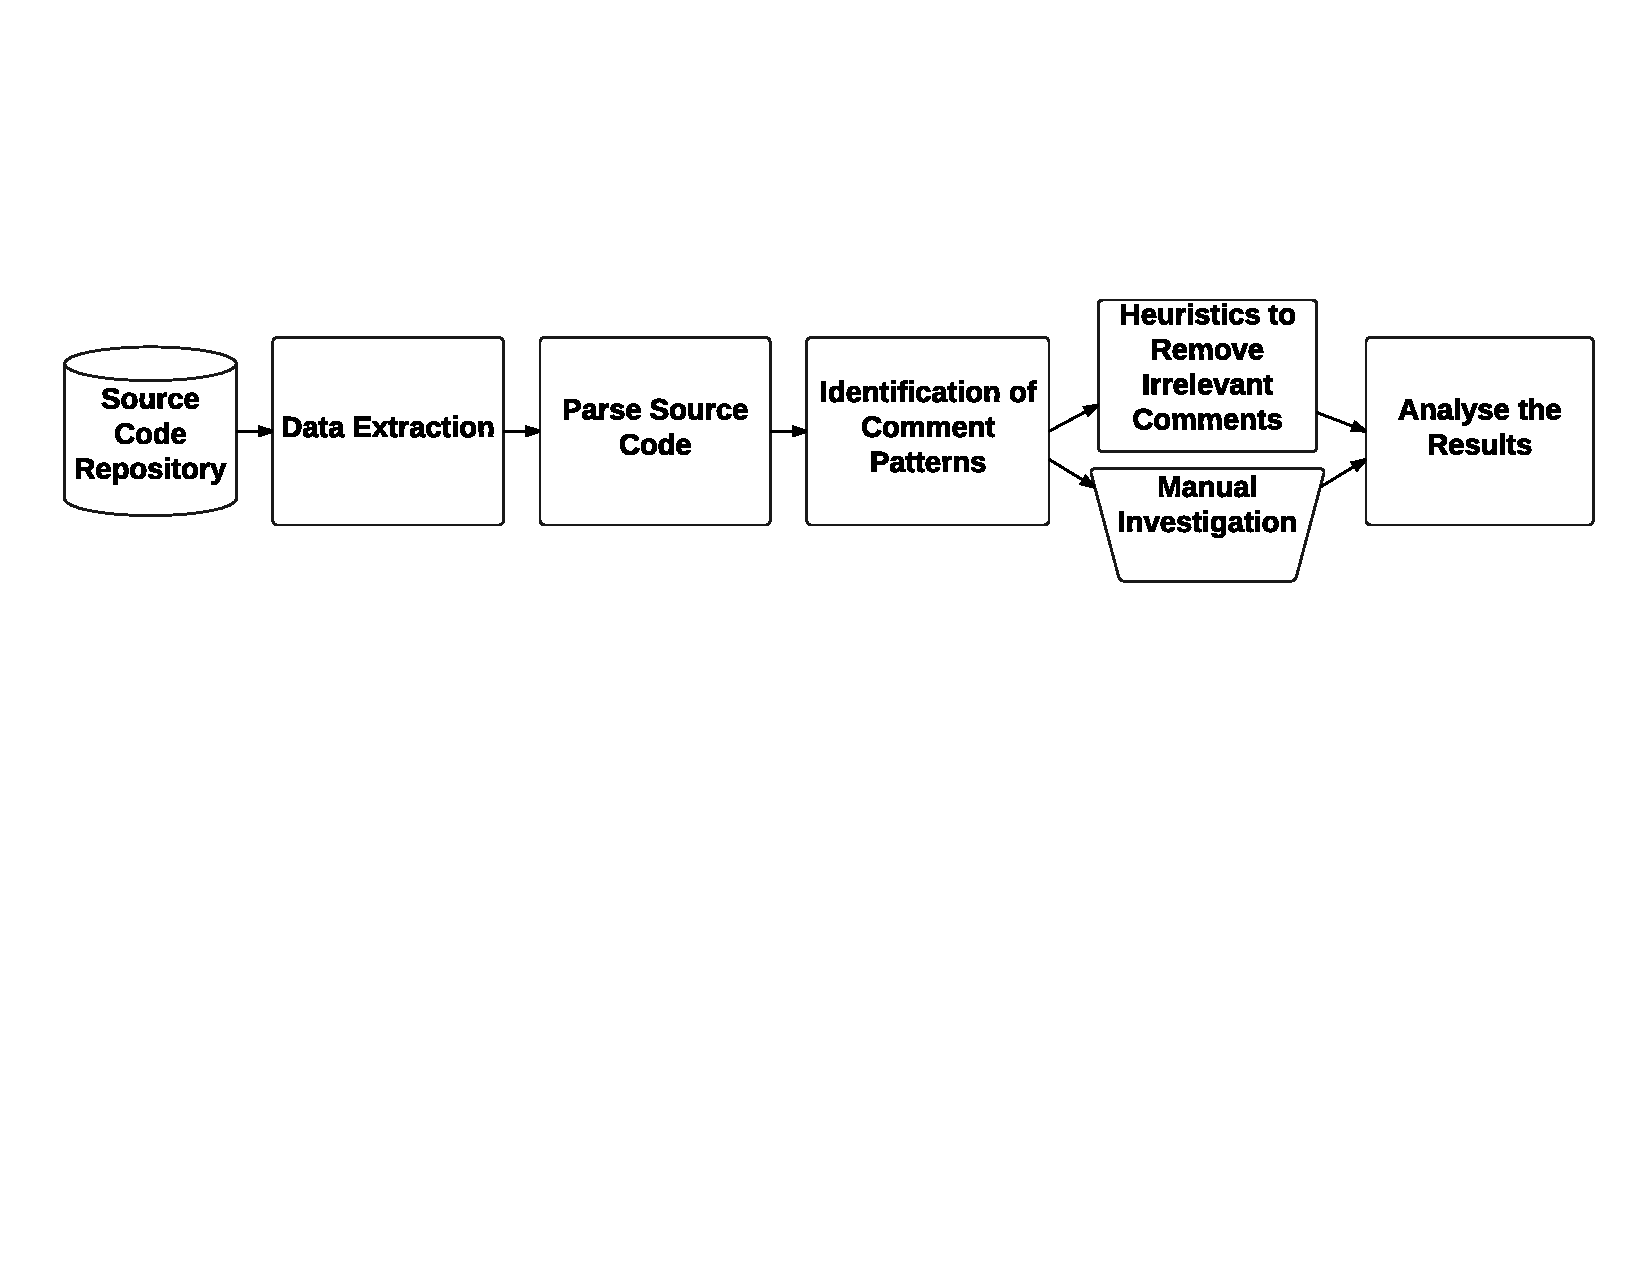
\includegraphics[width=1\textwidth]{figures/Approach2}
	%Caption goes below the figure
	\vspace{-10mm}
	\caption{Approach overview}
\end{figure*}


In this paper, we build on the promising approach of using code comments to detect one of the most impacting types of debt, namely \emph{design technical debt}, which we call \SADTD. We manually examine more than 17,000 code comments to extract comment patterns that can be used to detect \SADTD. To examine the effectiveness of our approach, we perform an empirical study on ten open source projects. Finally, we compare our approach to state-of-the-art approaches and examine the effectiveness of using automated refactoring techniques in mitigating \SADTD.

Based on our manual examination of the code comments, we derive 176 different comment patterns that can be used to detect \SADTD. These patterns are able to detect \SADTD with a precision ranging in 74.0-96.30\% and a recall ranging in 10.87-83.87\%. Moreover, we find that the design technical debt found with our approach is different than the design technical debt found using metric-based approaches~\cite{Zazworka2013CSE}. Finally, we find that automated refactoring can address up to 24.58\% of the methods containing \SADTD.

%Despite its utility this approach has one major limitation.
%There is no way to be sure that the detected code smells are indeed problems that the developers care about, and their resolution is absolutely necessary for the survival of the project.
%Many different refactorings opportunities can appear while analyzing a piece of source code, but it is still an open problem
%to determine the refactorings that should be recommended with higher priority, because they are more important for the developers.
%%Nikos: This is our big statement. I would even put it in emphasis
%\emph{Self-admitted design debt could be the missing element to guide the process of refactoring recommendation.}


%In particular, we would like to answer the following two research questions:
%
%\noindent\rqi 
%\everton{Explain in detail the different nature of each approach}
%We extracted 176 comment patterns that can identify \SADTD~in the source code.
%\nikos{The text that follows is ugly and unclear}
%While comparing the \SADTD~patterns with the more general Debt patterns, defined in \cite{Potdar2014ICSME}, we found that they have essentially different mechanics although some of the patterns that is found in one can also be found in the other one.
%All of the positive matches that the general Self-Admitted Technical Debt patterns generated was also contained in the \SADTD~ patterns matches. Which means that the more specific \SADTD~patterns made obsolete the general Self-Admitted Technical Debt patterns, regarding design debt. 
%
%\noindent\rqii
%\nikos{The same here! It's not even clear how we computed precision and recall}
%We find that our highest precision value has of 88.57\% in Squirrel SQL Client project and our lowest mark was of 74.07\% in Columba project. We achieved an high overall precision of 84.93\%. The overall recall measured was of 19.01\% Therefore our highest result while measuring recall was of 27.16\% in Jmeter and our lowest result was 10.87\% in JFreeChart.


The rest of the paper is organized as follows:  Section~\ref{sec:motivating_example} presents a motivating example. Section~\ref{sec:approach} details our approach. We present our case study results in Section~\ref{sec:case_study_results}, followed by a discussion in Section \ref{sec:discussion}. Section~\ref{sec:related_work} presents the related work. The threats to validity of our work are discussed in Section~\ref{sec:threats_to_validity}. Section~\ref{sec:conclusion} lists the conclusions of our work.



\section{Motivating Example}
\label{sec:motivating_example}
As mentioned earlier, one of the first works on self-admitted technical debt was the work by Potdar and Shihab~\cite{Potdar2014ICSME}. Their work showed that it is possible to identify self-admitted technical debt using source code comments. However, in their work, Potdar and Shihab studied \textit{generic} technical debt, i.e., they did not discriminate between the different types of technical debt. For example, technical debt can be in the form of design debt, testing debt, defect debt, and documentation debt. 

Since our work focuses on \SADTD, we first examined the effectiveness of using the general comments used by Potdar and Shihab to detect design technical debt. We applied the comment patterns that we derived (which we present later in the paper) and the comment patterns from Potdar and Shihab on the studied open source projects. As expected, the results produced by the general comment patterns identified all types of technical debt, indicating the need for more specific comment patterns that can be used to effectively identify design technical debt.

To illustrate our point, we show some example comments flagged by Potdar and Shihab's approach in the first column of Table~\ref{tab:satdmotivation}. The second column of the table shows the comments that are detected by the comment patterns we propose in this paper, which focus on \SADTD. A comparison of the comments in Table~\ref{tab:satdmotivation} clearly shows that the more specific comment patterns detect design issues. 

This simple example shows that comment patterns that specifically target design technical debt are needed. Simply using the general comment patterns may yield unfavourable results. We elaborate more on the performance of using the general comment patterns to detect \SADTD in Section~\ref{sec:case_study_results}.

%Comparing the comments in the table \ref{tab:satdmotivation} with the comments in table \ref{tab:sadtdmotivation} it is clear  that the first approach would not make any distinction between different categories of technical debt like design debt. All of the comments listed is table \ref{tab:sadtdmotivation} are related with design debt in the other hand in table \ref{tab:satdmotivation} is not what happens. We also argue that identifying each specific category of technical debt is important since they are managed and corrected in different ways. 

\begin{table*}[!hbt]
	\begin{center}
		\caption{Example of General/Design Self-admitted Technical Debt Comments}
		\vspace{-2mm}
		\label{tab:satdmotivation}
		\begin{tabular}{ p{3in} | p{3in} } 
			\toprule
			\textbf{General Self-Admitted Technical Debt} &  \textbf{Self-Admitted Design Technical Debt}  \\ 
			\midrule
			\textit{remove this code once bug 62405 is fixed for the mainstream GTK} & \textit{This can lead to code smell, meh! Do we care}\\
			\textit{FIXME - This caching thing should not be here; it's brittle.} & \textit{This is an absurdly long method! Break it up.}\\
			\textit{FIXME compat: updateActionBars : should do something useful} & \textit{there should be an interface, instead of the 		AbstractMessageFolder}\\
			\textit{FIXME this does not actually set the default since it is the wrong} & \textit{rethink where exactly some of the following methods belong (GenModel or GenPackage)}\\
			\textit{TODO: - please add some javadoc - ugly classname also} & \textit{Cyclic dependency with PersistenceManager}\\

			%\textit{FIXME: this is killing at least SSE editors, see bug 318034} & \textit{hack to support dockable view title update replace with listener pattern}\\
			%\textit{FIXME: this is not 64-bit clean} & \textit{This is in the wrong place.  It's not profile specific. It needs to be moved to main XMI reading code. }\\
			%\textit{HACK. Calling super.read() installs a required preferences change listener.} & \textit{This appears unused.  If it's needed, the Model API should be enhanced to provide a method that does this directly.}\\
			%\textit{This test is problematic. It makes assumptions about the behavior} & \textit{What does the magic number 6000 represent here? Put it in an explanatory literal! }\\
			%\textit{TODO: Won't our use of PathComparator take care of uniqueness?} & \textit{Downcast to avoid using an interface?  Yuck.}\\
			%\textit{FIXME: why override if nobody uses?} & \textit{We should actually rework this class to not implement Parser}\\
			%\textit{not exist yet. Throws a CoreException if there is a problem} & \textit{unhappy about this being public ... is there a better way?}\\
			%\textit{TODO this is such a hack it is silly.  There are still cases for race conditions etc} & \textit{remove use of instanceof!}\\
			%\textit{KLUDGE!! Test commented out until bug 170353 is fixed...} & \textit{a design flaw, it doesn't update properly}\\
			\bottomrule
		\end{tabular}
	\end{center}
\end{table*}





\section{Approach}
\label{sec:approach}

The main goal of our study is to extract comment patterns that can be used to effectively identify \SADTD. Figure~\ref{fig:approach} shows an overview of our approach. The following subsections detail each step of our approach.
 
\subsection{Data Extraction}

To perform our study, we obtain the source of ten large open source projects, namely Apache Ant, Jakarta Jmeter, ArgoUML,  Columba, EMF, Hibernate, JEdit, JFreeChart, JRuby and SQuirrel SQL Client. We chose the aforementioned projects, since they belong to different domains, and vary in size (e.g., LOC), and in the number of contributors.

Table~\ref{tab:projDetails} provides statistics about each of the projects used in our study. In total, we obtained more than 258,878 comments, found in 16,249 files. We also include the release used, the number of classes, and the total lines of code (LOC). In our study, we only use the Java files to calculate the LOC. It is important to notice that the number of comments shown for each project does not represent the number of commented lines, but rather the number of individual line, block, and Javadoc comments. 


%All the projects were downloaded from their respective websites, except from ArgoUml that we extracted the latest version,at the date, from its repository.  
%It represents the number of identified comments by the parsing tool. For example, a block comment of 10 lines will be treated as one comment, the same applies for Javadoc comments. It Does not matter how long a block or Javadoc comment can be, it will be always be counted as a single comment by the tool.

%Specific details for each one the projects are provided in table \ref{tab:projDetails}, including the release of each one of them, the number of classes, the number of comments and the number of lines of code. As a reference, we also added the number of contributors reported at OpenHub.net \cite{Openhub:home}. 

\begin{table*}[!tbh]
	\begin{center}
		\caption{Case Study Project Details and Statistics}
		\vspace{-2mm}
		\label{tab:projDetails}
		\begin{tabular}{l| c c c c c | p{2.5in}}
			\toprule
			\textbf{Project} & \textbf{Release} & \textbf{LOC} & \textbf{Classes} & \textbf{Comments} & \textbf{Contributors} & \textbf{Description}                                                      
			\\ \midrule
			Apache Ant       & 1.7.0            & 115,881      & 1,475            & 21,587            & 70                    & A Java library and command-line tool to build Java applications.           \\
			Jakarta Jmeter   & 2.3.2            & 81,307       & 1,181            & 20,084            & 32                    & An application to measure performance and assert functional behavior.      \\
			ArgoUML          & 0.34             & 176,839      & 2,609            & 67,716            & 87                    & An UML modeling tool.                                                      \\
			Columba          & 1.4              & 100,200      & 1,711            & 33,895            & 9                     & A desktop email client written in Java.                                    \\
			EMF              & 2.4.1            & 228,191      & 1,458            & 25,229            & 28                    & Eclipse Modeling Framework.                                                \\
			Hibernate        & 3.3.2 GA         & 173,467      & 1,356            & 11,630            & 216                   & An Object Relational Mapping framework.                                    \\
			JEdit            & 4.2              & 88,583       & 800              & 1,6991            & 55                    & A light weight text editor.                                                \\
			JFreeChart       & 1.0.19           & 132,296      & 1,065            & 23,123            & 18                    & A Java library to display graphics and charts.                             \\
			JRuby            & 1.4.0            & 150,060      & 1,486            & 11,149            & 291                   & Is the implementation of the Ruby language using the Java Virtual Machine. \\
			SQuirrel         & 3.0.3            & 215,234      & 3,108            & 27,474            & 40                    & A graphical SQL client written in Java.                                    
			\\ \bottomrule
		\end{tabular}
	\end{center}
\end{table*}

 
\subsection{Parse Source Code}

After obtaining the source code of all projects, we extract the comments from their source code. We use JDeodorant~\cite{Tsantalis2008CSMR}, an open-source Eclipse plug-in, to parse the source code and extract the code comments. Once extracted, we store all comments in a relational database to facilitate the processing of the data.

%keep this information in memory while it executes source code analysis. We took advantage of the parsing functionality and developed our own version of the tool, that stores the parsed information of the comments in the database. We list the number of classes found and number of comments for each project in table \ref{tab:projDetails}. In order parse the code properly, it is necessary that all analyzed projects can be compiled and built in the Eclipse environment. 

\subsection{Identification of \SADTD~Comment Patterns}
Once we store all comments in the database, our next step is to identify the \SADTD~comment patterns. Since we are dealing with natural language in the comments, it is challenging to automatically determine what comments indicate design technical debt. Therefore, we opted to use two different approaches to determine comment patterns that indicate design technical debt. First, we use the terms mentioned in prior work~\cite{fowler1999refactoring,brown1998antipatterns,martin2009clean} (i.e., code smell and anti-pattern names) as indicators of design problems to determine comments that are indicative of design technical debt. Second, we manually examined and classified all  comments of one project i.e., Apache Ant, in order to determine comment patterns that are indicative of \SADTD. After analyzing the results, we found that combining comment patterns from the two aforementioned approaches provides the best results. We detail the steps taken to achieve each of the two approaches.

%\noindent \textbf{Using well-known terms to identify \SADTD comments}
%
%To create the Design Technical Debt patterns we took advantage of the design flaws names that can be found in Fowler's book \cite{fowler1999refactoring}, Brown et al book \cite{brown1998antipatterns} and Martin's book \cite{martin2009clean}. Based on the words extracted from these books and our experience, we searched for synonyms in the database. The first step is verify if the selected word has a match in the database, then we read all the comments related to it. Doing so, we were able to identify new words and more than that, understand the frequency that this word is used as \SADTD. 
%Following this approach we were able to come up with three different dictionaries for patterns to find \SADTD comments. 
%  
%The first group of patterns we called the ``-ilities'' patterns. It possesses words like ``Configurability'', ``Security'', etc. It contains 17 words and in our preliminary analysis we matched 181 comments. After a quick inspection we kept 14 of these comments as potential \SADTD comments. The following are examples of the kept comments: \textit{ ``Apparently in some environments you can't catch the security exception at all... will probably have to work around''} and \textit{``pretty weak and don't provide real security.''}.
% 
%We based the second group of patterns in the names of well-know bad smells and anti-patterns like ``Clone'',``Dead'', etc. Using these patterns we found the following potential  \SADTD comments in the source code: \textit{``this class is considered to be dead code by the Ant developers and is unmaintained. Don't use it''}. The anti-patterns patterns contains 8 words, in our preliminary analysis we matched 1,316 comments and after a quick inspection we kept 148 of these comments.
%
%The last group of patterns we put the words that can be related with Design such as: ``Ambiguous'', ``Avoid'', ``Big'', etc. We found 3,449 matches using 14 different words. Of those we kept 196. The following are examples of the kept comments:\textit{``...find a way to avoid the cost of creating a String here''}. 
%
%At the end of this step, we were able to come up with three different dictionaries for patterns to find \SADTD comments.
%
%To test the performance of the dictionaries we have quantified the number of comments that matches with any of the words contained in one of the dictionaries, then we did a quick manual examination to inspect the results obtained. The manual inspection done in this phase took about 8 hours. 
%
%Using the three group of patterns we matched 4,946 comments. Out of that we classified 358 comments as potential \SADTD comments.
%To classify the comment as a potential \SADTD comment we read trough the 4,946 comments where patterns matched the words in the comment and then we  eliminated the matches that clearly did not represent a \SADTD. 
%
%During this analysis we notice that the number of matches is way higher than the number of \SADTD. Which means that we are obtaining a high number of false positives. To mitigate this problem we took action in two dimensions: the comments and the \SADTD patterns. First, we need to eliminate comments that are irrelevant and second, we need to improve our \SADTD patterns to be more precise. 

\subsubsection{Applying Heuristics to Eliminate Irrelevant Comments}

When applying our first approach, i.e., using the terms in the prior work to identify comments that are indicative of \SADTD, we found that we are able to flag comments that indicate design issues, but also flag many false positives. We analyzed the false positives to see whether we can gain any insight into why they appear and how we can eliminate them. 

We identified three main types of false positives. First, license comments, containing copyright information and legal rights. Second, commented source code containing Java keywords, e.g., ``big'' and ``long''. Finally, Javadoc comments were flagged, however, they often had no relation to design issues. As a result, we came up with three heuristics and a post-processing step to reduce the number of false positives.

\begin{table*}[!hbt]
	\begin{center}
		\caption{Number of Comments After the Application of Each Heuristic}
		\vspace{-2mm}
		\label{tab:heuristicDetails}
		\begin{tabular}{l| p{.6in} p{.6in} p{.8in} p{.7in} p{.55in}} 
			\toprule
			\textbf{Project} & 	\textbf{Initial no. of Comments} & \textbf{After license heuristic} &  \textbf{After comment code heuristic}  &  \textbf{After Javadoc heuristic} & \textbf{After post processing} \\ 
			\midrule
			Apache Ant & 21,587 & 20,421 & 20,268 & 6,239 & 4,436 \\ 
			Jakarta Jmeter & 20,084& 18,840 & 18,530 & 12,360 & 8,126 \\
			ArgoUML & 67,716 & 28,180 & 27,848 & 13,972 & 10,303 \\
			Columba & 33,895 & 14,600 & 14,256 & 9,095 & 6,825 \\
			EMF & 25,229 & 24,355 & 24,093 & 8,861 & 5,868 \\
			Hibernate  & 11,630 & 10,446 & 10,277 & 4,908 & 3,071 \\
			JEdit & 16,991 & 16,128 & 16,037 & 13,118 & 11,232 \\
			JFreeChart & 23,123 & 22,114 & 22,047 & 5,902 & 4,449 \\
			JRuby & 11,149 & 10,274 & 10,080 & 6,887 & 5,176 \\
			SQuirrel  & 27,474& 25,566 & 25,196 & 13,713 & 8,627 \\  
			\bottomrule
		\end{tabular}
	\end{center}
\end{table*}
  
 
\begin{itemize}


\item{\textbf{Heuristic to remove license comments.}} 
When license comments are added to the Java files in a project they are generally placed in the first lines of the file, before the class declaration. Based on this knowledge we created a heuristic that eliminates comments that are placed before the class declaration. To validate the result of this heuristic we examined a sample of the comments being removed to check if they were indeed license comments. We noticed that some comments were placed before the class declaration although they were not license comments. To mitigate the risk of eliminating important comments, we added one more condition: If the comment contains one of the task-reserved words (e.g. ``todo'', ``fixme'', or ``xxx'') we do not remove the comment.

\item{\textbf{Heuristic to remove commented source code.}}
If a commented piece of source code contains Java keywords like ``long'' or ``big'', it will increase the number of false positives of our approach. Commented source code can be found for several different reasons. One of the possibilities could be that the code is not being currently used, or if the particular piece of code is used to debug the program. Since commented code does not have \SADTD, we remove commented source code using a regular expressions that captures typical Java code structures.

\item{\textbf{Heuristic to remove Javadoc comments.}}
The Javadoc comments contain information about the purpose and use of methods and classes. That said, Javadoc comments rarely mention \SADTD. Therefore, we create a heuristic that removes Javadoc comments. To mitigate the risk of eliminating some correct cases, we added one exception - if the comment contains one of the task-reserved words (e.g. ``todo'', ``fixme'', or ``xxx'') we keep that Javadoc comment. 

%We argue that since these comments appear in the public documentation of projects, it is less likely that a developer will add a \SADTD~comment there. 
\item{\textbf{Post processing technique to merge multiple line comments}}
Another problem that we found while analyzing the comments was that some times developers make long comments, using multiple single-line comments instead of a Block comment. Treating every single line of a long comment as an individual comment causes us to miss important context details that could be recovered by treating all single-line comments as a single block comment. Therefore, we create a post processing technique that searches for consecutive single-line comments and groups them. 

\end{itemize}

The steps mentioned above significantly reduced the number of comments in our dataset and helped us focus on the most applicable and insightful comments. For example, in the Apache Ant project, applying the above steps helped reduce the number of comments from 21,587 to 4,436 comments.


\subsubsection{Manual investigation of identified \SADTD~comments} 
%Once we understand the pattens in the one dataset, we can add then to our \SADTD patterns. The first necessary step to do that is to create the dataset, as to the best of our knowledge, there is none available to the date. We choose one of the projects to manually classify all comments and create this dataset, the selected project was Apache Ant. 

In addition to using the words that indicate design issues to detect \SADTD, we also manually examine our dataset to extract comment patterns that indicate~\SADTD~comments. We started by examining all of the 4,436 comments for the Apache Ant project and classified each comment as being related to \SADTD or not. Since our focus in this work is on design debt, comments related to other types of technical debt were not labeled as \SADTD comments. The classification of the Apache Ant comments took approximately 32 hours and was performed by the first author of the paper.

\noindent \textbf{Manual Examination of Comments to Identify \SADTD~Comment Patterns}

In the end of the classification we identified 93 \SADTD~related comments out of 4,436 comments in Apache Ant project.

Our next goal was to abstract the comments and come up with a set of \emph{comment patterns} that indicate \SADTD. Comment patterns are general patterns that represent one or more comments. Simply using a single word to identify \SADTD~comments can be misleading since the context that the word appears in can completely change the meaning of that word. In order to address this issue, we take into consideration some of the other words that appear in the same sentence to combine them into what we call comment patterns. 

%To create comment patterns, we combine multiple \SADTD~words, so that some context is considered.

% with word task indicators ones, (e.g, ``todo'', ``fixme'', ``xxx'') in addition to the expressions that we were creating observing the \SADTD comments in the dataset. 

%For every new \SADTD comment pattern that was created we manually sample the results in two different databases, one had all the comments for Apache Ant and the other one had all the comments for all the remaining projects. While exploring the results we notice that small variations in the expression used to find  \SADTD comments can improve the results. For example we apply the patterns ``place some where else'' and ``move somewhere else'' to identify misplaced code.

By the end of this step, we had identified the comment patterns that indicate \SADTD. \textbf{In total, we had 176 comment patterns that can be used to detect \SADTD}. To facilitate future work in the area, we make our dataset and the comment patterns publicly available \footnote{http://users.encs.concordia.ca/~e\_silvam/publications.html}. 

Table \ref{tab:dictionarySample} provides a sample of the comment patterns that we used to identify \SADTD~comments. 
%The first column of Table~\ref{tab:dictionarySample} shows  the type of design issue and the second column shows the \SADTD~ comment pattern capturing the corresponding design issue. 
The `\%' symbol indicates that the pattern uses the SQL language wildcards. Wildcards make the query to match anything before or after the wildcard symbol. For example, ``dependen\%'' would result in positive results for comments that contains the words ``dependency'' or ``dependencies''.

\begin{table}[t!]
	\begin{center}
		\caption{Sample \SADTD Comment Patterns}
		\vspace{-2mm}
		\label{tab:dictionarySample}
		\begin{tabular}{ c }
			\toprule
			\textbf{Related Comment Patterns} \\ 
			\midrule
			     `\%future\%may\%'       \\
			     `\%future\%better\%'  \\
			     `\%future\%enhance\%' \\ 
			     `\%future\%change\%'  \\  	
			 `\%dependency\%cycle\%'  \\
			 `\%todo\%dependenc\%'    \\
			 `\%fixme\%dependenc\%'   \\
			 `\%xxx\%dependenc\%'    \\
			\bottomrule		 		
		\end{tabular}
	\end{center}	
\end{table}


Once we derive the 176 comment patterns that indicate \SADTD, we use these patterns to answer our research questions, which we detail in the next section.


%\subsection{Applying Comment Patterns and Measuring their Performance}
%\label{sec:applying_comment_patterns_measuring_performance}
%We conduct an experiment to measure the performance of our approach using precision and recall. \emph{Precision} measures how many of the comments flagged using our comment patterns are indeed \SADTD. \emph{Recall} measures how many of the comments indicating \SADTD~our approach can catch. To measure recall we first needed to classify a dataset and labeling all of the \SADTD~comments of the project. Since measuring recall is a difficult and time consuming task, we report recall values for three projects, Apache Ant, Jakarta Jmeter and JFreeChart.
%
%We measure first the results of the three first dictionaries, ``-ilities'', ``design'' and ``bad smells''. As our first classified dataset was Apache Ant, we use it to measure precision and recall of the dictionaries. 

%Table \ref{tab:dictionaryEvaluation} shows the results for each one of the dictionaries found analyzing the Apache Ant dataset, which has 93 \SADTD comments. When running the ``-ilities'' patterns we found 10 matches of which 2 were classified  as \SADTD comments. That represents a precision of 20\% and recall of 2.15\%.  Using the Design patterns we found 54 matches of which 5 were classified  as \SADTD comments. For the Bad Smell patterns we found 39 matches and 1 \SADTD comment. The precision and recall for these dictionaries were 9.26\% , 5.38\% and 2.56\% , 1.01\% respectively. 

%The performance of the three dictionaries was not in the desired level yet, and as we analyze the \SADTD comments from Apache Ant we notice that expressions patterns represents better our desired dataset than single words patterns. We created then expressions for the three dictionaries combining their words with task specific ones like ``todo'',``fixme'' and ``xxx''. 

%As a result we come up with a unified expression group of patterns that have expressions based on the three previous group of patterns and expressions based on the \SADTD comments of Apache Ant project. The performance of this new group of pattern can be found in details in Table \ref{tab:expressiondictionary_precision} and Table \ref{tab:expressiondictionary_recall}. For Apache Ant we got 96.30\% precision and 83.87\% recall. For Jakarta Jmeter we found 75 matches of that 66 were \SADTD comments, the recall as of 27.16\%. JFreeChart we found 12 matches out of that 10 was classified as \SADTD comments. The recall for JFreeChart was 10.87\%.

%Finally we measured performance for the other seven projects remaining to be analyzed. As it is necessary to classify the dataset to measure recall, and this task is very time consuming, we did not classify them due time constrains. The precision achieved considering the comments of all projects was of 85.86\%. We found 964 comments out of 825 \SADTD comments.

\section{Case study Results}
\label{sec:case_study_results}

The goal of our study is develop an effective way to detect \SADTD. To do so, we first derive comment patterns that can be used to detect \SADTD (RQ1). Then, we examine the effectiveness of the derived comment patterns in detecting \SADTD in real-life open source projects (RQ2). We detail the motivation, approach and present the results of each of our research questions in the remainder of this section.

%We perform an exploratory study using the data of ten open source projects namely - Apache Ant, Jakarta Jmeter, ArgoUML, Columba, EMF, Hibernate, JEdit, JFreeChart, JRuby and SQuirrel SQL Client. Our first question is related to the patterns to identify \SADTD~comments. 

\rqi

\noindent \textbf{Motivation:} 
Prior work has shown that comments, embedded in the source code, are a good indicator of technical debt~\cite{Potdar2014ICSME}. However, the prior work did not discriminate between the different types of debt. Since we know that design technical debt is one of the most impactful types of technical debt~\cite{Marinescu2012IBM}, we would like to derive specific comment patterns that are indicative of design technical debt.

%know that there are different categories under the big umbrella that technical debt represents \cite{Alves2014MTD},so we would like to propose comment patterns that are specific to design debt as it is mentioned as the kind of debt that has most impact in software quality \cite{Marinescu2012IBM}. Therefore, our first task is to derive a set of comment patterns that indicate \SADTD~comments.

\noindent \textbf{Approach:} Our general approach to derive the \SADTD comment patterns was detailed in Section~\ref{sec:approach}. In a nutshell, we start by using common words that are indicative of design issues listed in prior work (e.g.,~\cite{fowler1999refactoring, brown1998antipatterns,martin2009clean}). Since using these words returns many irrelevant comments (e.g., licensing and Javadoc comments), we use a number of heuristics to reduce the number of comments so that the most relevant comments are returned. Finally, we perform a manual examination to derive the final list of 176 comment patterns that best indicate \SADTD.

Once we have the comment patterns, we apply them on ten open source projects namely - Apache Ant, Jakarta Jmeter, ArgoUML, Columba, EMF, Hibernate, JEdit, JFreeChart, JRuby and SQuirrel SQL Client - in order to determine what comments are flagged and how common the different comment patterns indicate \SADTD. 

Furthermore, we compare the similarity of the comments detected using the comment patterns we derive in this paper to the \emph{generic} comment patterns proposed in prior work~\cite{Potdar2014ICSME}. To do so, we manually read the comments of three projects (i.e., Apache Ant, Jmeter and JFreeChart\footnote{Note: since this analysis required us to manually examine and label each comment, we only performed this analysis on three of the ten projects.}) and labeled each comment as a design technical debt related comment or not. Then, we used our comment patterns and the generic comment patterns from prior work to detect the labeled design technical debt comments. Finally, to see how different (or similar) the comment patterns are, we report the amount of overlap for each of the three projects.

%To determine what comment patterns best indicate \SADTD, we applied the approach shown in ~\ref{sec:approach}. In a nut shell, we started by using common words that prior work~\cite{fowler1999refactoring, brown1998antipatterns,martin2009clean} associated with design paradigms (e.g., ``Clone", ``Bad Smell", ``Duplicated", etc). Since using this list did not yield favorable results, we manually examined source code comments of the Apache Ant project. To minimize the large cost of manual examination, we used a number of heuristics that reduced the set of comments to inspect to a reasonable set. 

%In total, the Apache Ant project 21,587 comments across 1,475 Java classes. After applying our heuristics, we ended up with a total of 4,678 comments that required manual inspection. Doing the manual inspection we identified 93 \SADTD~comments. By analyzing the common patterns in this dataset, we ended up with a final list of 175 \SADTD~patterns. The entire process of determining these \SADTD~comment patterns took one masters student (the first author) approximately 32 hours to complete. 
 

\noindent \textbf{Results:} 
In total, we derived 176 different comment patterns that indicate \SADTD. Table~\ref{tab:topperformingpatterns} shows the ten top most common comment patterns that indicate \SADTD~in all projects. The first column of Table~\ref{tab:topperformingpatterns} lists the comment pattern and the second column lists the frequency that the comment pattern matched one of the manually labeled design technical debt comments in the three studied projects. From the table, we observe that ``hack'' is the most common pattern, followed by ``todo+remove'' and so on. It is important to note here that Table~\ref{tab:topperformingpatterns} only lists the top ten most common patterns, we provide a full list of all the 176 comment patterns in \footnote{http://users.encs.concordia.ca/~e\_silvam/publications.html}.

When we examined the comment patterns derived in our paper and the general comment patterns from the prior work, we noticed a significant difference. However, we also noticed some similarities. For example, the comment pattern ``hack'' shows up in both, our design specific comment patterns and the generic comment patterns. Therefore, to compare how different (or similar) the two approaches are, we applied both approaches on the three projects with the manually labeled comments.

Table~\ref{tab:approach_comparisson} shows the number of comments that indicate design technical debt (second column), the number of comments flagged by our comment patterns (third column), the number of comments flagged by the generic comment patterns (fourth column), and the overlap between the comments flagged by both approaches. First, we find that our approach flags more \SADTD comments, with the exception of JFreeChart. Second, we notice that the overlap is small, but close to the number of comments flagged by the generic comment patterns. This means that in most cases, the comments flagged by the generic comment patterns will be covered by the comments flagged using our approach, since the overlap is close to the generic comment patterns value.


%In total, we determined a total of 175 unique comment patterns. We first present the pattern that we applied, including the wild cards that give our patterns more flexibility in the search. Then we shown the number of \SADTD~comments that were found in Ant project for each pattern, including the percentage that each one represents from the total found. 


\begin{table}[t]
	\begin{center}
		\caption{The Top Ten Most Common \SADTD Comment Patterns Across All Ten Projects}
		\vspace{-2mm}
		\label{tab:topperformingpatterns}
		\begin{tabular}{l| c  c}
			\toprule
			\textbf{Pattern}          & \textbf{Number of occurrences} & \textbf{Percentage} \\ 
			\midrule
			`\%hack\%'                    & 32                             & 19.75\%             \\
           		 `\%not \%sure \%'             & 9                              & 5.56\%              \\
          		  `\%should\%instead\%'         & 9                              & 5.56\%              \\
          		  `\%todo\%remove\%'            & 8                              & 4.94\%              \\
          		  `\%ugly\%'                    & 6                              & 3.70\%              \\
            		`\% fix for \%'               & 6                              & 3.70\%              \\
            		`\%why\%not\%'                & 6                              & 3.70\%              \\
            		`\%todo\%duplicat\%'          & 5                              & 3.09\%              \\
           		 `\%todo\%public\%'            & 5                              & 3.09\%              \\
           		 `\%idea?\%'                   & 4                              & 2.47\%              \\
            \bottomrule
		\end{tabular}
	\end{center}
\end{table}


\begin{table*}[!hbt]
	\begin{center}
		\caption{Comparing the Use of Design-Specific Comment Patterns and the Generic Comment Patterns in Detecting \SADTD}
		\vspace{-2mm}
		\label{tab:approach_comparisson}
		\begin{tabular}{l| p{1in} p{1in} p{1.2in} p{1in}  }
			\toprule
			\textbf{Project} &\textbf{Total \# of Design Comments} &\textbf{\# of Comments Our Approach Flags} &\textbf{\# of Comments Generic Approach Flags} &\textbf{Overlap}  \\ 
			\midrule
			Apache Ant      & 93 & 78 & 16 & 13   \\
			Jakarta Jmeter  & 243 & 66 & 24 & 23   \\
			JFreeChart      & 92 & 10 & 13 & 5  \\
			\bottomrule
		\end{tabular}
	\end{center}
\end{table*}

%\begin{table}[!hbt]
%	\begin{center}
%		\caption{Sample of General Self-Admitted TD patterns VS Sample of Design Self-Admitted TD}
%		\label{tab:general_vs_sadtd}
%		\begin{tabular}{l|l}
%			\toprule
%			\textbf{General Self-Admitted TD} & \textbf{Design Self-Admitted TD} \\ 
%			\midrule
%			this is uncool                    & `\%hack\%'                       \\
%			risk of this blowing up           & `\%todo\%remove\%'               \\
%			remove this code                  & `\%not \%sure \%'                \\
%			something's gone wrong            & `\%why\%not\%'                   \\
%			certainly buggy                   & `\%should\%instead\%'            \\
%			treat this as a soft error        & `\%todo\%dependenc\%'            \\
%			probably a bug                    & `\%better\%way\%'                \\
%			this isn't very solid             & `\%ugly\%'                       \\
%			is this line really safe          & `\%todo\%public\%'               \\
%			something serious is wrong        & `\%for\%some\%reason\%'          \\ 
%			\bottomrule
%		\end{tabular}
%	\end{center}
%\end{table}

%\everton{Elaborate the discussion between the differences of Self-Admitted design techinical debt patterns and the general Self-Admitted techinical debt patterns. DESIGN vs GENERAL and Phrases vs Patterns  }
%We also compare the comment patterns derived here to the more general comment patterns derived by Potdar and Shihab~\cite{Potdar2014ICSME} used to determine self-admitted technical debt in general (i.e., design debt, defect debt, testing debt and so forth). Comparing to Table \ref{tab:general_vs_sadtd}, the comment patterns indicating \SADTD~are different. This observation shows that although comments are good indicators of self-admitted technical debt \cite{Potdar2014ICSME}, different types of technical debt are indicated by different comment patterns.
%\everton{Add more discussion about the nature of the comments}

%We also evaluated the performance of both approaches in 3 projects, as shown in Table \ref{tab:approach_comparisson}. In the table we present the number of false positives and true positives for each approach. False positives (FP) represent the number of comments that were identified but is not \SADTD. True positives (TP) represents the number of comments that were identified and were indeed a \SADTD. We also present the overlap between the comments found by each approach. Finally we calculate the total of comments that can be found by both approaches, by the summing the TP's and subtracting the overlap. Then we calculate the percentage of \SADTD~comments found for each approach. In the only case that the General Self-Admitted TD approach perform better than the Design Self-Admitted TD approach is in JFreeChart, at cost of precision.  

%In addition to determining the comment patterns that indicate \SADTD, we also investigated the most common \SADTD~comment patterns. Our findings show that the top 5 most common \SADTD~comment patterns are: ``hack" 15.1\%, ``todo+remove" 11.5\%,``not+sure" 6\%, ``why+not" 4\% and ``should+instead" 3.6\% . We see that the top 5 most common comment patterns indicate almost the majority of the \SADTD, accounting for more than 40\% of the \SADTD~occurrences. 

To perform this analysis we took in consideration all the matches that each of the patterns retrieve. It's possible that one or more patterns match the same comment.

\conclusionbox{We find that the top 5 most common comment patterns are: hack, not+sure, should+instead, todo+remove and ugly. The comment patterns proposed in our approach flag more \SADTD compared to the generic comment patterns proposed in prior work.}
\vspace{0.3in}

%\begin{table*}[!hbt]
%	\begin{center}
%		\caption{Approach comparison between General Self-Admitted TD and Design Self-Admitted TD}
%		\label{tab:approach_comparisson}
%		\begin{tabular}{l| c c c c c c }
%			\toprule
%			\textbf{Project} &\textbf{FP+TP/TP Design} &\textbf{FP+TP/TP General} &\textbf{Overlap} &\textbf{TP Union} & \textbf{Design} & \textbf{General} \\ 
%			\midrule
%			Apache Ant      & 81/78 & 31/16 & 13  & 81  & 96.29\% & 19.75\%   \\
%			Jakarta Jmeter  & 75/66 & 46/24 & 23  & 67  & 98.51\% & 35.82\%   \\
%			JFreeChart      & 12/10 & 77/13 & 5   & 18  & 55.55\% & 72.22\%   \\ 
%			\bottomrule
%		\end{tabular}
%	\end{center}
%\end{table*}

\rqii

\noindent \textbf{Motivation:} After deriving the comment patterns to detect \SADTD, one of the first questions that comes to mind is - how effective are the proposed comment patterns in detecting \SADTD. Determining the effectiveness of the comment patterns will give us confidence in their ability to detect \SADTD in software projects.

%After identifying the \SADTD~patterns we address our second research question, about evaluating the performance of our patterns in means of precision and recall. We manually examined the comments to determine design debt. However, we need to determine the effectiveness of these patterns. If the patterns are too general, then we will have many false positives leading to a waste of effort. If it is too restrictive, then we will miss many of the actual \SADTD. Therefore, our goal here is to find out how well our \SADTD~comment patterns do at detecting \SADTD.

\par \noindent \textbf{Approach:} To measure the effectiveness of our proposed comment patterns in detecting \SADTD, we use the common measure of precision and recall. Precision measures how many of the comments our patterns flag as being \SADTD, actually are \SADTD. To calculate precision, we apply the 176 comment patterns to all the comments in the ten projects and then manually determine which of the flagged comments are actually \SADTD. Recall measures how many of the actual \SADTD in each project, our comment patterns are able to detect. To calculate recall, we apply our comment patterns on the three projects that we manually classified each comment for. Then, we measure the percentage of all the comments that are actually \SADTD comments (true occurrences) that were detected by our comment patterns. Since the calculation of recall requires that we read each comment manually, we only calculate the recall for three of the ten projects.




%First we evaluate the precision of the \SADTD~patterns. We want to assert how many of the comments found by our patterns really represents a \SADTD. First, we developed a simple Java program to match the patterns of the expression dictionary with the comments in the database. Then, as there is no automated way to identify if a comment is in fact a \SADTD~comment, we manually assert the results. We repeated these steps to determine the precision of our \SADTD~patterns for each project. 

%The next step is to evaluate recall. Supposing that you know all of \SADTD~comments existent in a project, recall is measured by comparing the number of \SADTD~comments that the approach was able to find out of the total number of \SADTD~comments existent in the project. Then, this number is represented as a percentage. As mentioned before, the necessary dataset to conduct this evaluation needs to be created as there is none available to the best of our knowledge. Therefore, we manually classified all the comments of two more projects namely - Jakarta Jmeter and JFreeChart in addition to the already classified Apache Ant. As manual classification of all comments is a very time consuming task, we limited our classification to these three projects. However, these projects represents different application domains and therefore, we considered as a good sample of the analyzed projects. We classified   8,102 comments in Jakarta Jmeter project and 4,452 comments in JFreeChart project. The first author took 54 and 29 hours respectively to create the classified dataset for this experiment. 

%Finally, we evaluate recall analyzing the number of found \SADTD~comments with the total number of \SADTD~comments in the classified datasets. While measuring precision and recall we just take in consideration the total number of unique \SADTD~comments matched. For example, if two different \SADTD~patterns matches the same comment we consider as one unique \SADTD~comment instead of two. 

\noindent \textbf{Results:} Table~\ref{tab:precision_and_recall} shows the precision and recall values of our approach. As explained earlier, since recall required the manual examination of all code comments, we only present the recall of three of the ten projects. We observe that the precision values for all the projects is good, ranging between 74.07-96.30\%. However, the recall values are not as high, ranging between 10.87-83.87\%. It is important to note here that the highest precision and recall values are achieved for Apache Ant, which is the project we mainly used to derive the comment patterns.

The consistently high precision values show that our comment patterns have a low false positive rate, i.e., comments flagged using our comment patterns are most likely \SADTD. However, the low recall values (on the projects other than Apache Ant) indicate that our comment patterns will not flag all the \emph{actual} comments indicating \SADTD. In a nutshell, our comment patterns tend to be more conservative, reducing wasted effort, however the price to pay is that we may miss some of the \SADTD comments in the code. 

To better understand the reason for the low recall values, we manually investigated some of the comments that indicate \SADTD in Jmeter and JFreeChart and found that some projects use project specific comment conventions that our comment patterns miss to capture. For example, in JFreeChart most of the \SADTD comments were preceded with a ``FIXME:''. That said, the high recall value achieved for Apache Ant shows that high recall values are achievable, however, one needs to examine and take into account the specific comment conventions used in that specific project. In the future, we plan to use Natural Language Processing techniques in order to derive comment patterns that may be applied across projects to detect \SADTD.
%First we shown how many matches we got for each project and then we present the result of the manual assertion of each one of the \SADTD~comments. In general, our approach had achieved precision higher than 80\% for the majority of the projects. Without taking into consideration Apache Ant, which a high precision was already expected (96.30\%), our highest precision value has of 88.57\% in Squirrel SQL Client project and our lowest mark was of 74.07\% in Columba project. We achieved an high overall precision of 84.93\% considering all projects analyzed except Apache Ant. 

%We present the recall of our approach in Table \ref{tab:expressiondictionary_recall}, for each classified dataset that we have - Apache Ant, Jakarta Jmeter and JFreeChart - we show the total number of \SADTD~comments, the number of matches that really represent a \SADTD~found by our approach as the true positives and the calculated recall percentage. The overall recall measured was of 19.01\% as we are not taking Apache Ant in consideration as it was used to come up with the expression dictionary at first place. Therefore our highest result while measuring recall was of 27.16\% in Jmeter and our lowest result was 10.87\% in JFreeChart.

%We consider that the perfect result would be achieving hight values in both of the measured dimensions, precision and recall. What happens in the majority of times though, is that one can always improve one of the dimension while willing to sacrifice the other one. We argue that for our approach the same principle can be applied. We achieved a high overall precision (84.93\%) and a low overall recall (19.01\%). 

\conclusionbox{Our comment patterns can detect \SADTD comments with a precision between 74.07-96.30\% and a recall between 10.87-83.87\%.}

%We also consider that one possible way to improve recall without significantly losing precision is to apply natural language processing techniques to improve the approach once that is possible to see that the combination of certain words into \SADTD patterns has a high precision matching \SADTD comments.

\begin{table}[!hbt]
	\begin{center}
		\caption{Precision and Recall of Our Approach}
		\label{tab:precision_and_recall}
		\begin{tabular}{l| c c c }
			\toprule
			\textbf{Project} & \textbf{Precision} & \textbf{Recall}\\ 
			\midrule
			Apache Ant        & 96.30\%  &    83.87\%      \\
			Jakarta Jmeter   & 88.00\%  &    27.16\%      \\
			JFreeChart         & 83.33\%  &    10.87\%      \\
			ArgoUML            & 88.05\%  &       -   \\
			Columba             & 74.07\%  &       -   \\
			EMF                    & 85.18\%  &       -   \\
			Hibernate            & 87.18\%  &       -   \\
			JEdit                    & 81.92\%  &       -   \\
			JRuby                  & 88.07\%  &       -   \\
			SQuirrel               & 88.57\%  &       -   \\
			\bottomrule
		\end{tabular}
	\end{center}
\end{table}

%\begin{table}[!hbt]
%	\begin{center}
%		\caption{Expression dictionary recall}
%		\label{tab:expressiondictionary_recall}
%		\begin{tabular}{l| c c c}
%			\toprule
%			\textbf{Project} & \textbf{All TP} & \textbf{Found TP} & \textbf{Recall} \\ 
%			\midrule
%			Apache Ant       & 93           & 78                      & 83.87\%         \\
%			Jakarta Jmeter   & 243          & 66                      & 27.16\%         \\
%			JFreeChart       & 92           & 10                      & 10.87\%         \\ 
%			\bottomrule
%		\end{tabular}
%	\end{center}
%\end{table}


%\begin{table}[!hbt]
%	\begin{center}
%		\caption{Dictionaries Evaluation}
%		\label{tab:dictionaryEvaluation}
%		\begin{tabular}{l| c c c c} 
%			\toprule
%			\textbf{Dictionary}  & \textbf{Found} &  \textbf{Match}  &  \textbf{Precision} & \textbf{Recall} \\ 
%			\midrule
%			``-ilities'' & 10 & 2 & 20\% & 2.15\% \\ 
%			Design & 54 & 5 & 9.26\% & 5.38\% \\
%			Bad Smell  & 39 & 1 & 2.56\% & 1.01\% \\ 
%			\bottomrule
%		\end{tabular}
%	\end{center}
%\end{table}


\section{Discussion}
\label{sec:discussion}
\begin{figure*}[!thb]
  \centering
  \subfigure[Design Debt]{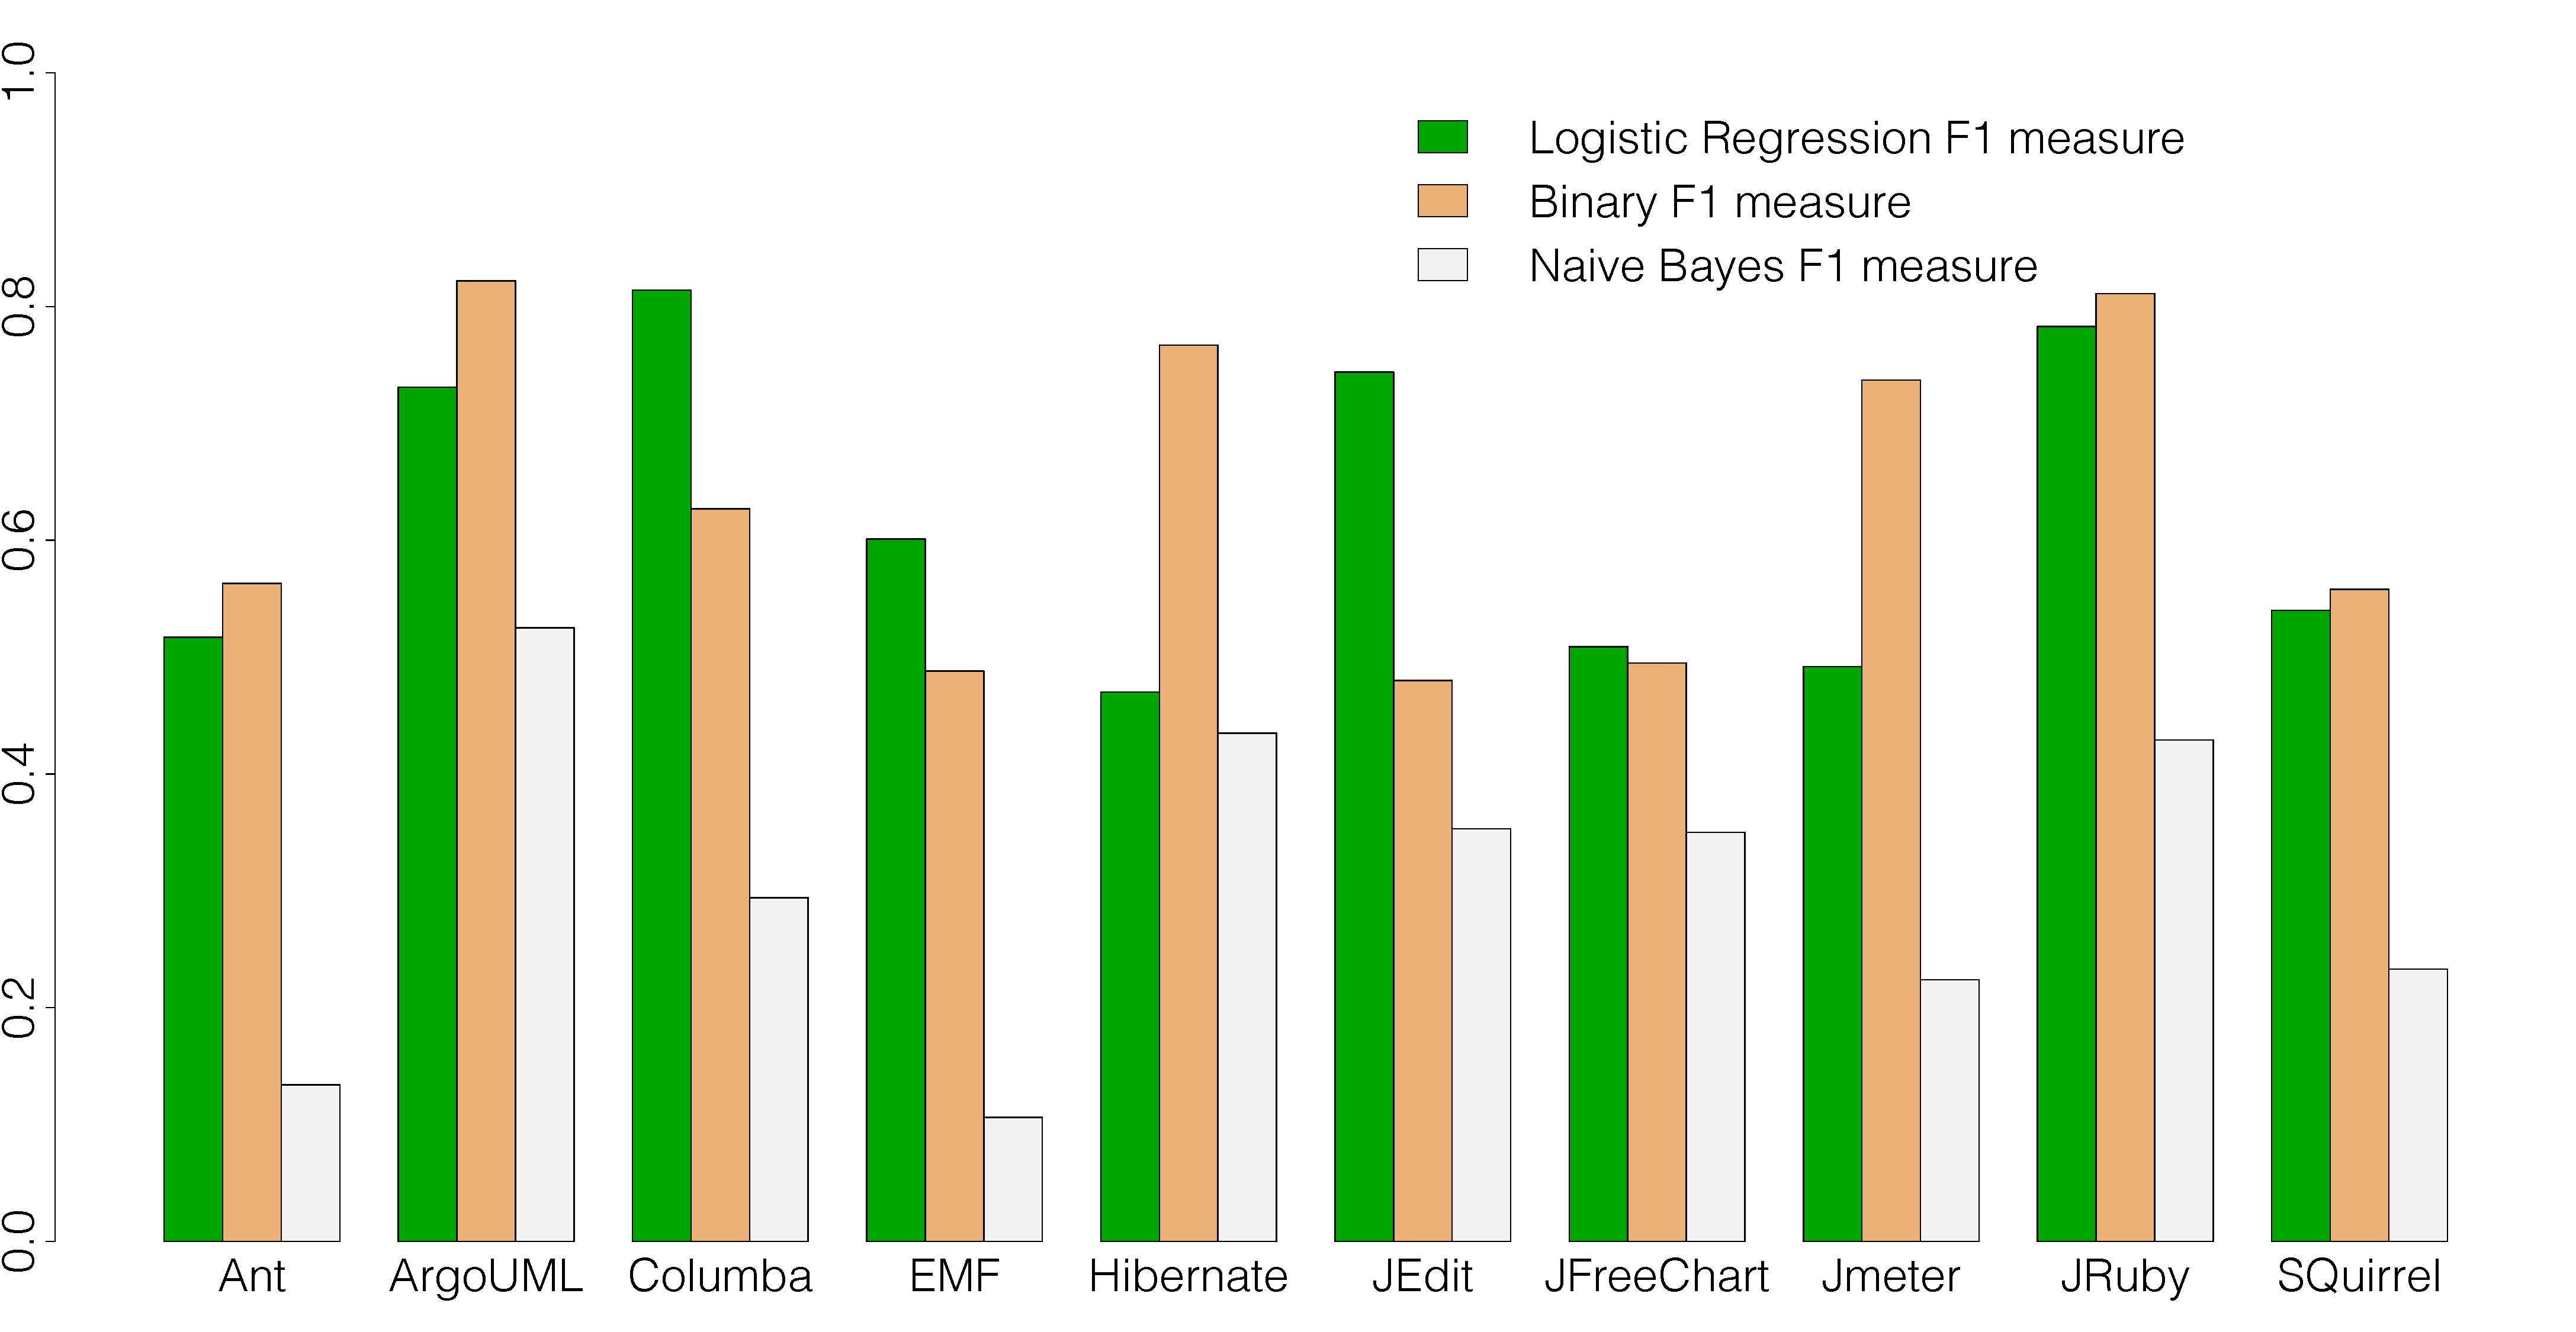
\includegraphics[width=0.48\textwidth]{figures/classifier_algorithms_comparison_design.pdf}
  \label{fig:algorithms_comparison_design}}
  \subfigure[Requirement Debt]{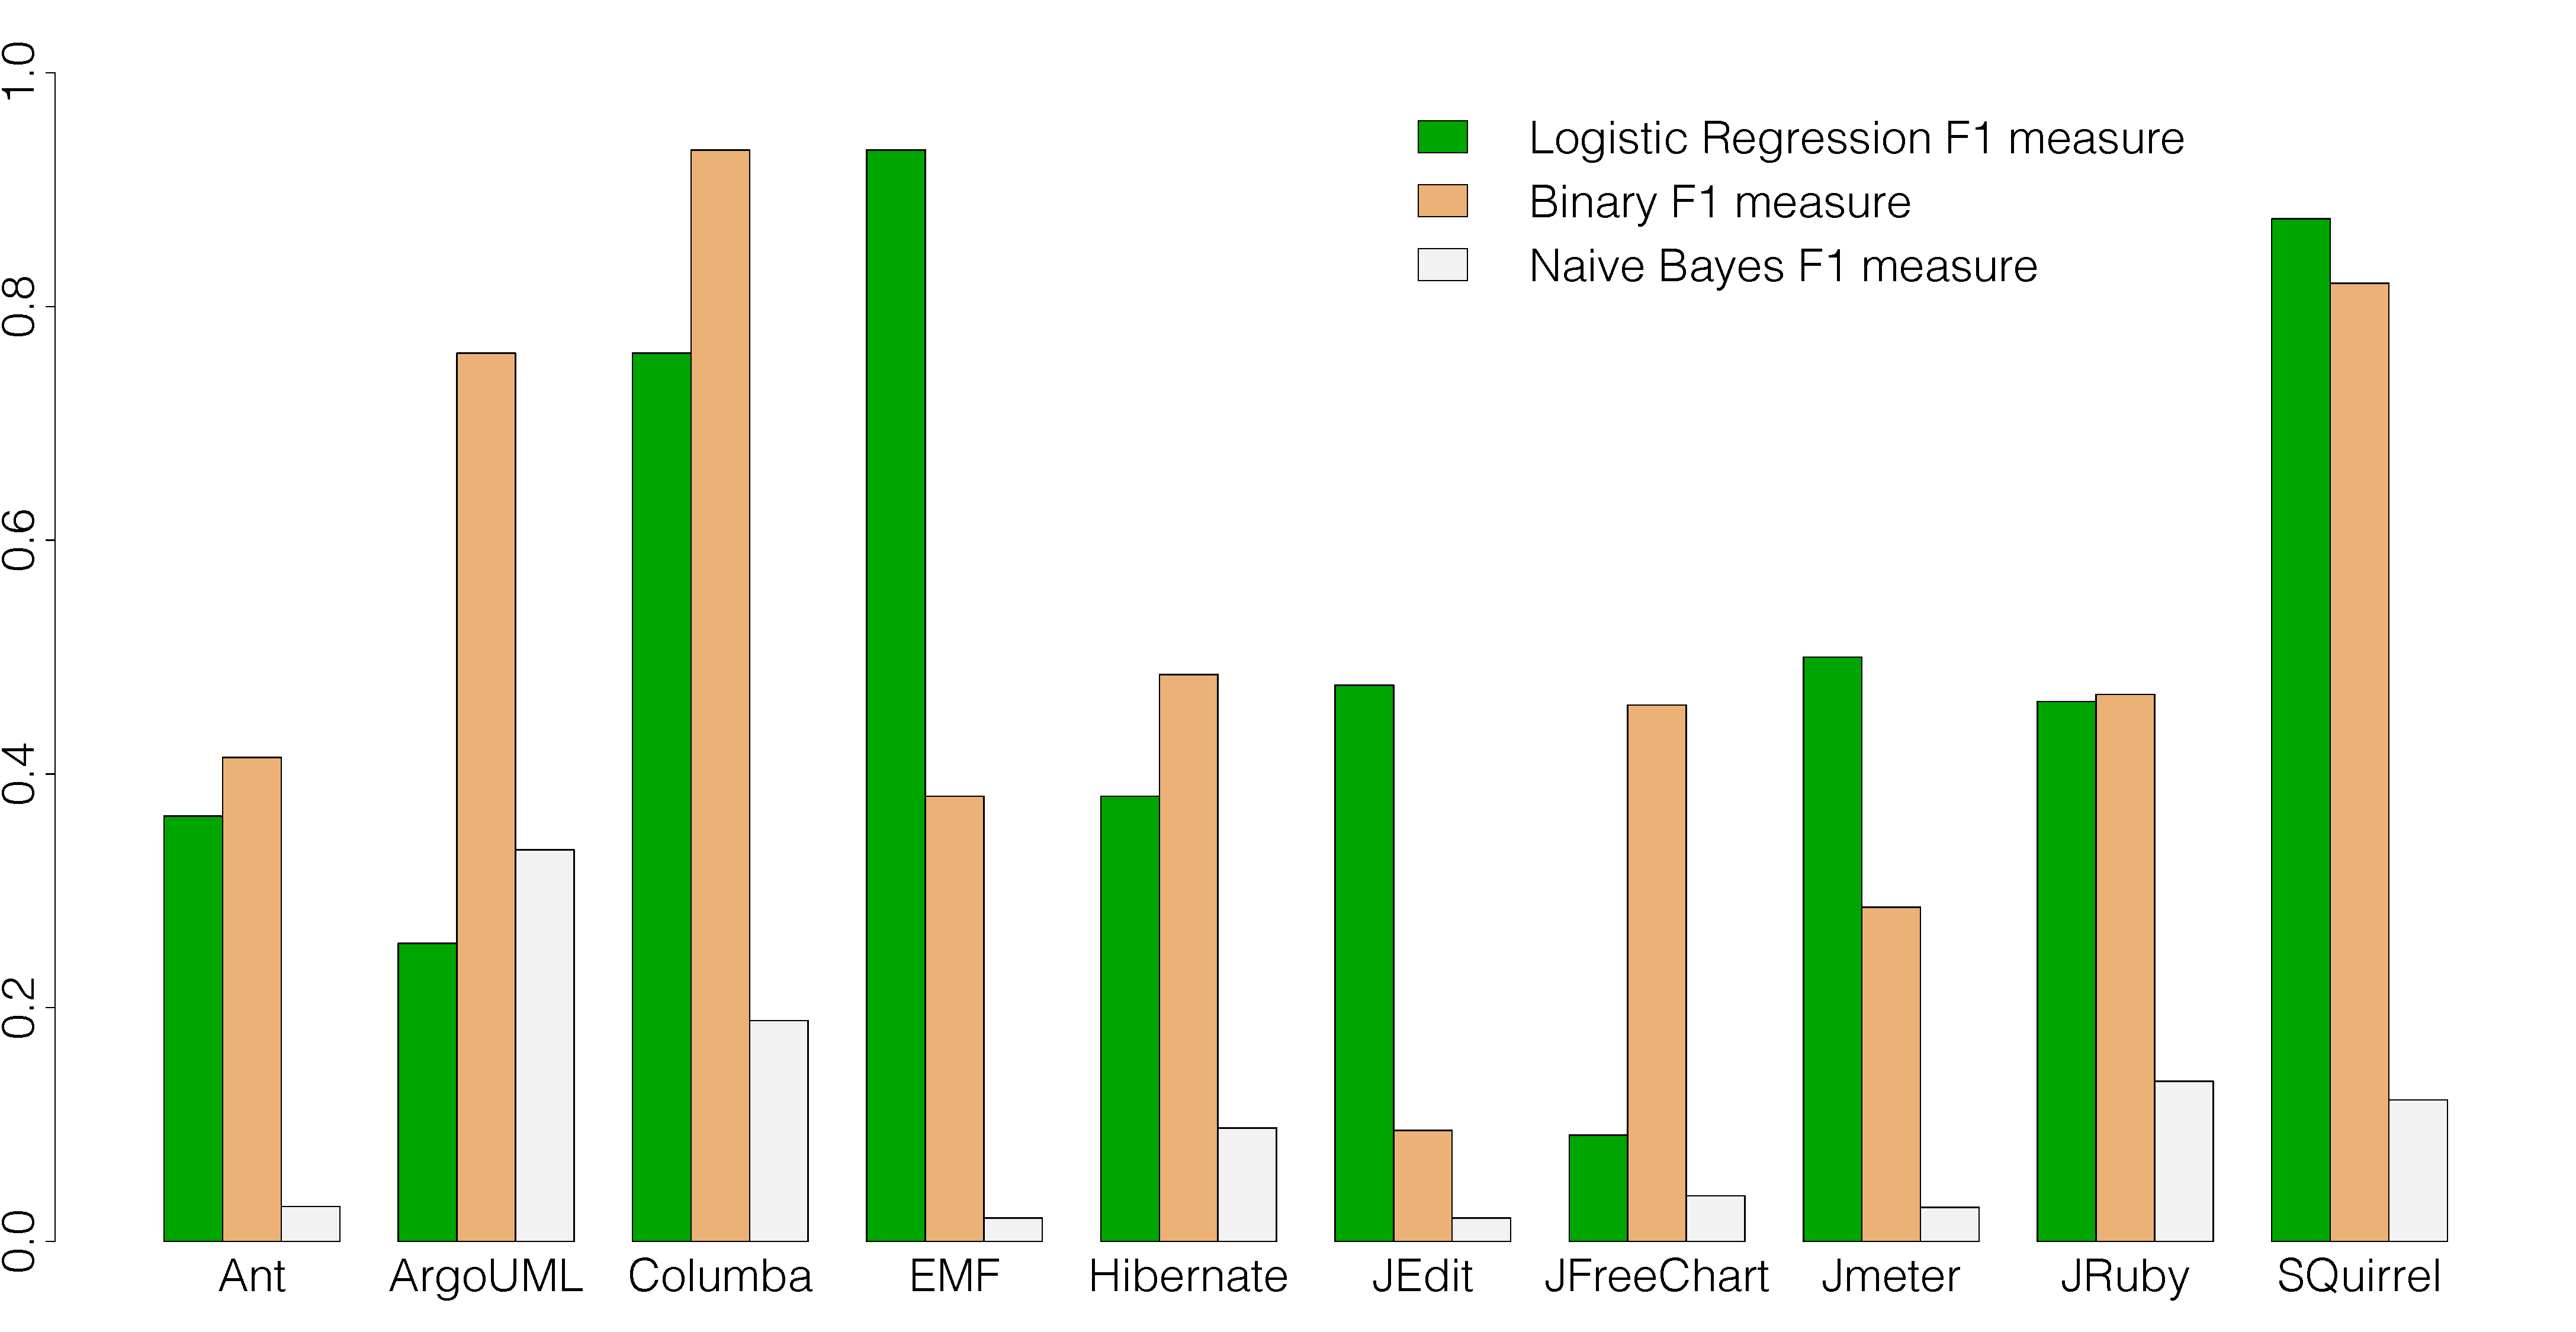
\includegraphics[width=0.48\textwidth]{figures/classifier_algorithms_comparison_requirement.pdf}
  \label{fig:algorithms_comparison_requirement}}
  \caption{Classification algorithms performance comparison}
  \label{fig:algorithms_comparison}
\end{figure*}

In this paper we propose an approach to identify \SATD comments using the Stanford Classifier. This tool, once trained correctly, can automatically classify natural language text. We create a training dataset of \SATD comments and analyzed the classification performance across ten open source projects. In RQ1, we show that our approach can outperform the current state-of-the-art in 10 out of 10 projects while identifying design and requirement debt. However, is not clear the reason why our approach was not equally effective across all projects. For example, JEdit has the worst F1 measure of all projects while classifying requirement \SATD.

\subsection{Investigating Outlier Projects}
By investigating JEdit comments, we notice two main reasons: first, the project has 10,322 comments. Of those only 14 are requirement \SATD. The data distribution represents a challenge to the classification. Even though the dataset is very unbalanced our precision was 0.125, which compared with the random classifier baseline precision of 0.001, shows that our approach is still much more useful. Second, most requirement \SATD comments in this project are in the middle of long comments. Since our approach create a high number of prediction features for \SATD comments and also for without technical debt comments, long comments have more chances to match a higher number of without technical debt features. Therefore, long comments can generate `noise' that hinders the classification performance. One possible way to reduce this effect is through the addition of more similar data, as the addition of more similar data can change the prediction features generated by the classifier. 

\emad{I do not see the point of the 2 paragraphs below}

\emad{begin: remove} Intuitively we know that each project has its own particularities, and that each group of developers, must often, create a unique way to communicate their concerns with each other. This unique trait of source code comments is inherited from the natural language itself and renders the fully automated prediction of every single \SATD very unlikely. Even when analyzing a old aged project, changes in the context of the application and turnover of developers can reflect changes in the way that source code comments are written. We can notice the impact of these particularities on the detailed performance analysis conducted in RQ3, where we can notice that the addition of more comments can eventually decrease the F1 measure performance.


For a great portion of \SATD comments there are common traits. Words as `workaround', `hack' are commonly imbued with criticism and the developers sense that this is not the appropriate solution for the problem in hand. However, relying just in these words for the identification of \SATD is not good enough as shown in Figures \ref{fig:f1_measure_comparison_design_debt} and \ref{fig:f1_measure_comparison_requirement_debt}. Therefore, NLP techniques, as proposed in our work, are needed in order to effectively identify \SATD comments.
\emad{end: remove}

\subsection{Investigating the Impact of the Underlying Classifier of the NLP Classification}

In our work, all the classification done by the Stanford Classifier used a Logistic Regression classifier. However, would be interesting to see how other  algorithms perform when classifying our dataset. Then, we choose two other algorithms to execute the classification with: Naive Bayes generative classifier and Binary classifier.

Figures \ref{fig:algorithms_comparison_design} and \ref{fig:algorithms_comparison_requirement} compare the performance between the three different algorithms. We find that the Naive Bayes has the eorst average F1-measure of 0.308 and 0.058 for design and requirement technical debt, respectively. The reason behind the low F1-measure average is that the Naive Bayes algorithm favors recall at the expense of precision \emad{we need a citation for this claim}. For example, while classifying design debt, the average recall was of 0.847 and precision 0.195. The two other algorithms present more balanced results compared to Naive Bayes, and the difference in performance between them is not as accentuate. The Logistic Regression classifier achieved F1-measures of 0.620 and 0.403, while the binary classifier F1-measures for design and requirement \SATD is 0.634 and 0.400, respectively. 

Although the Binary classification has a slightly better performance, for our research purpose, the Logistical Regression algorithm provide more insightful features as outcome. These features were analyzed and presented in RQ2. 

\subsection{Textual Similarity for Design and Requirement Debt}
%\begin{figure*}[!thb]
  \centering
  \subfigure[Design Debt]{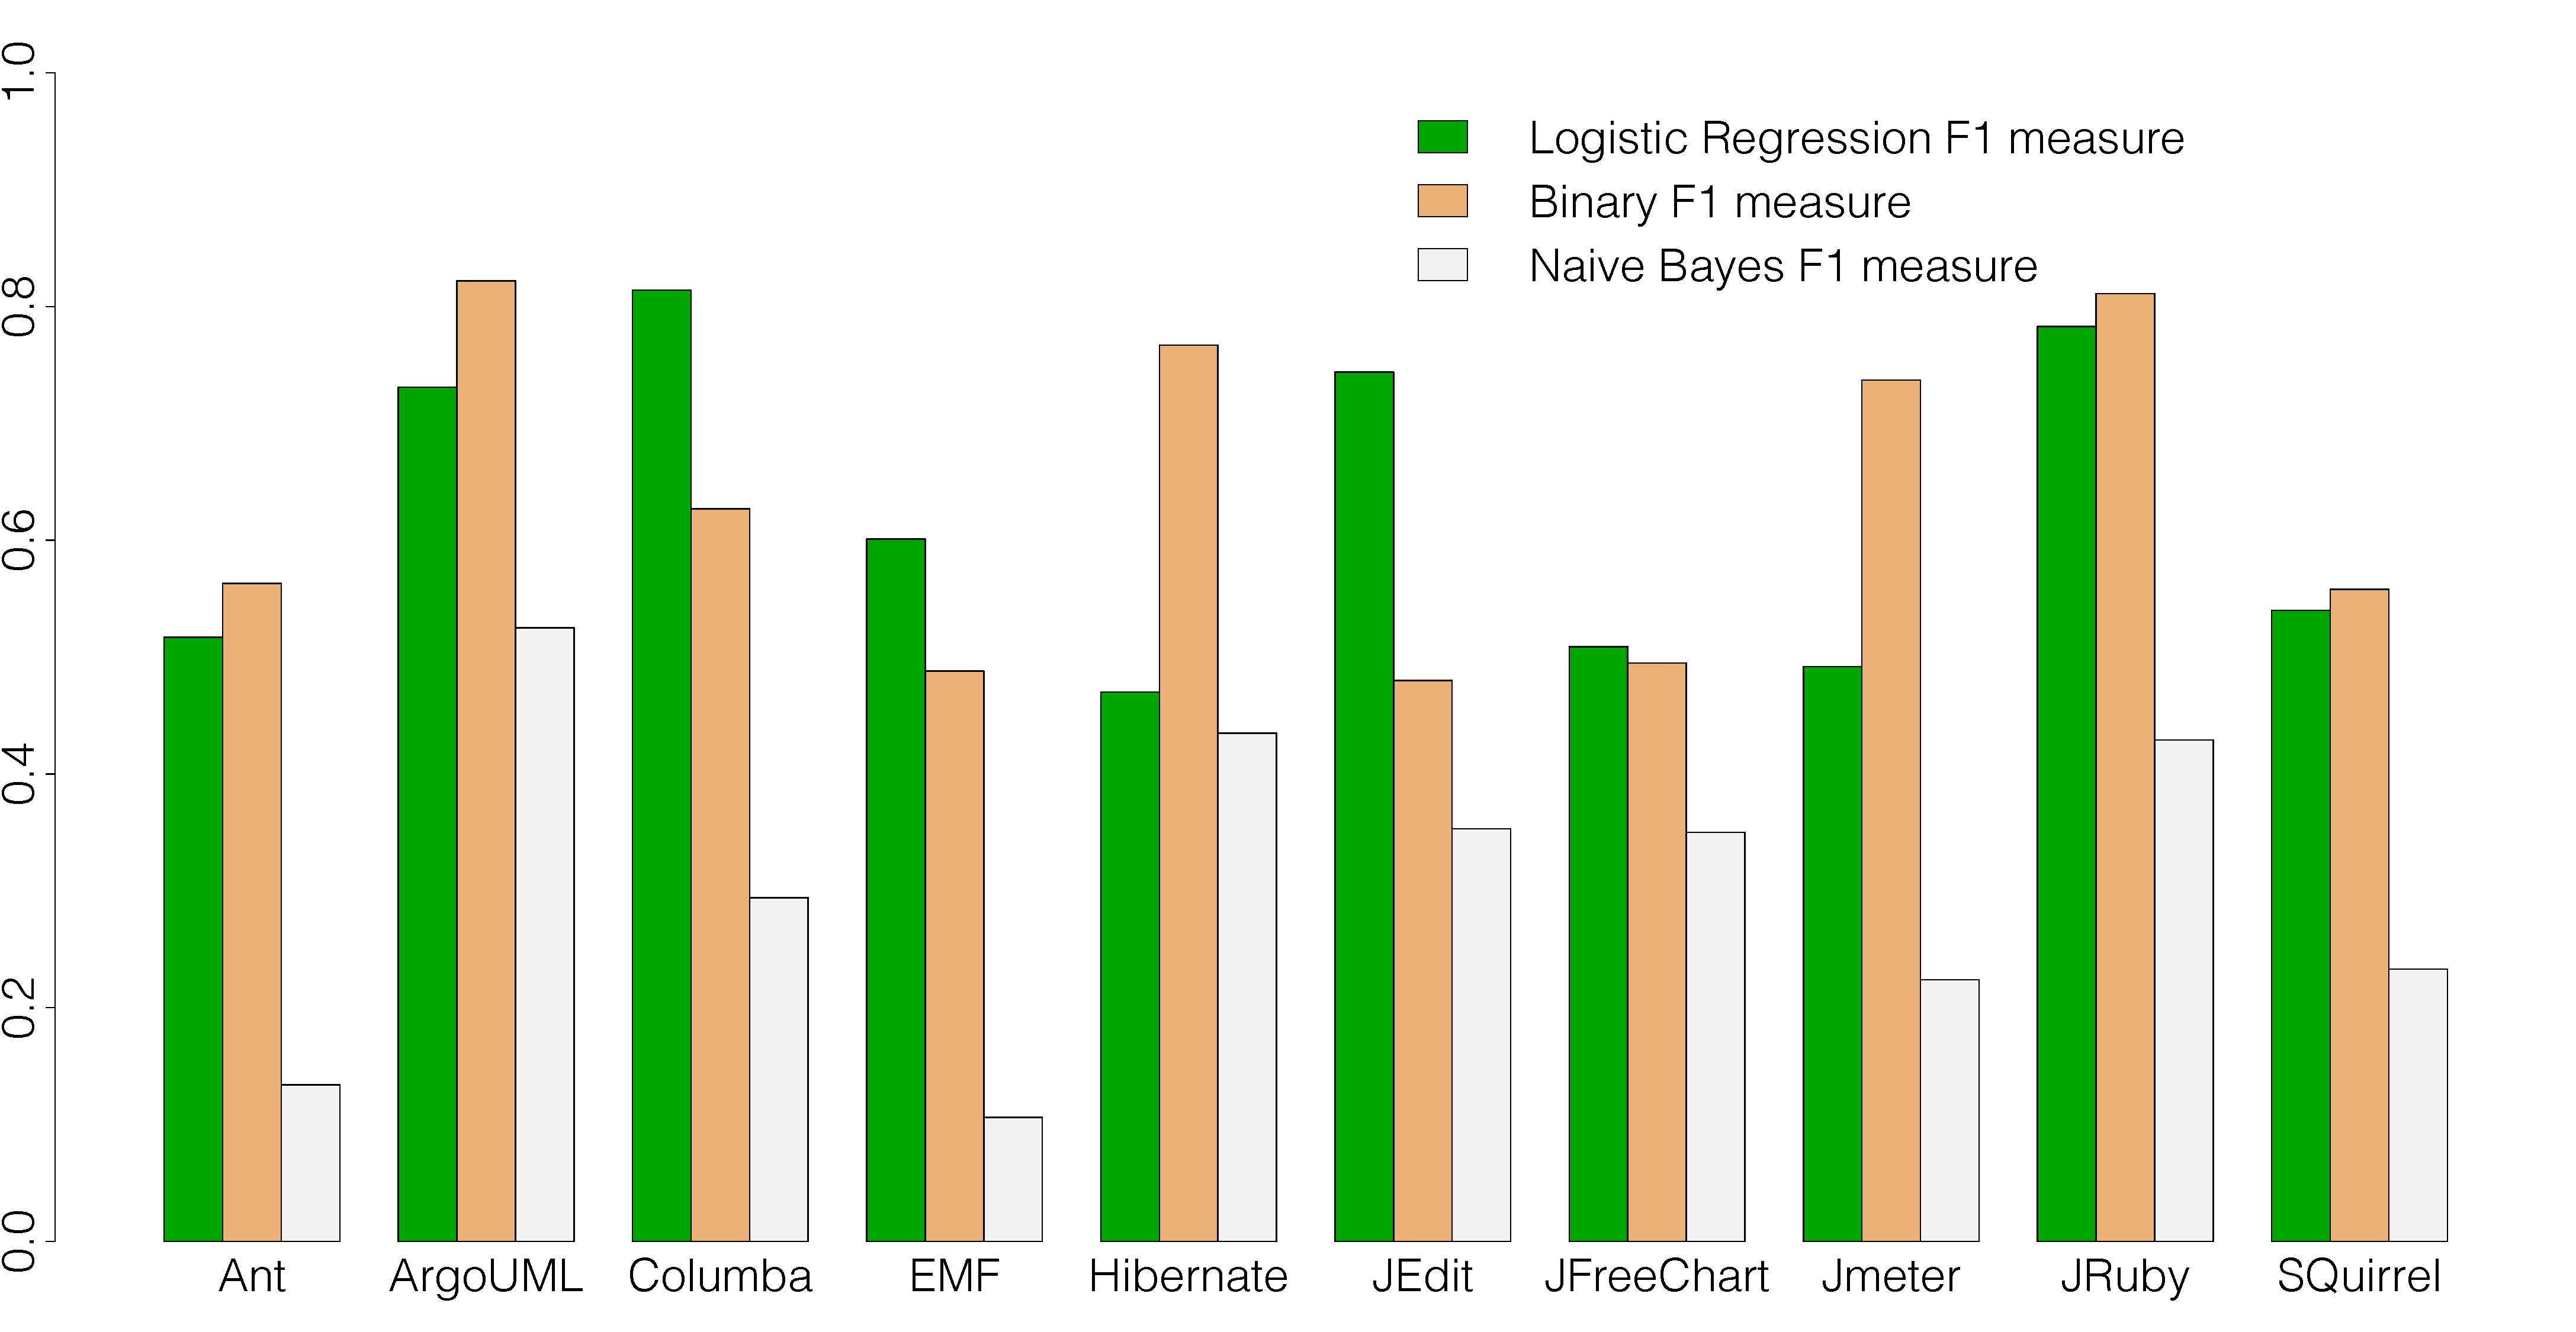
\includegraphics[width=0.48\textwidth]{figures/classifier_algorithms_comparison_design.pdf}
  \label{fig:algorithms_comparison_design}}
  \subfigure[Requirement Debt]{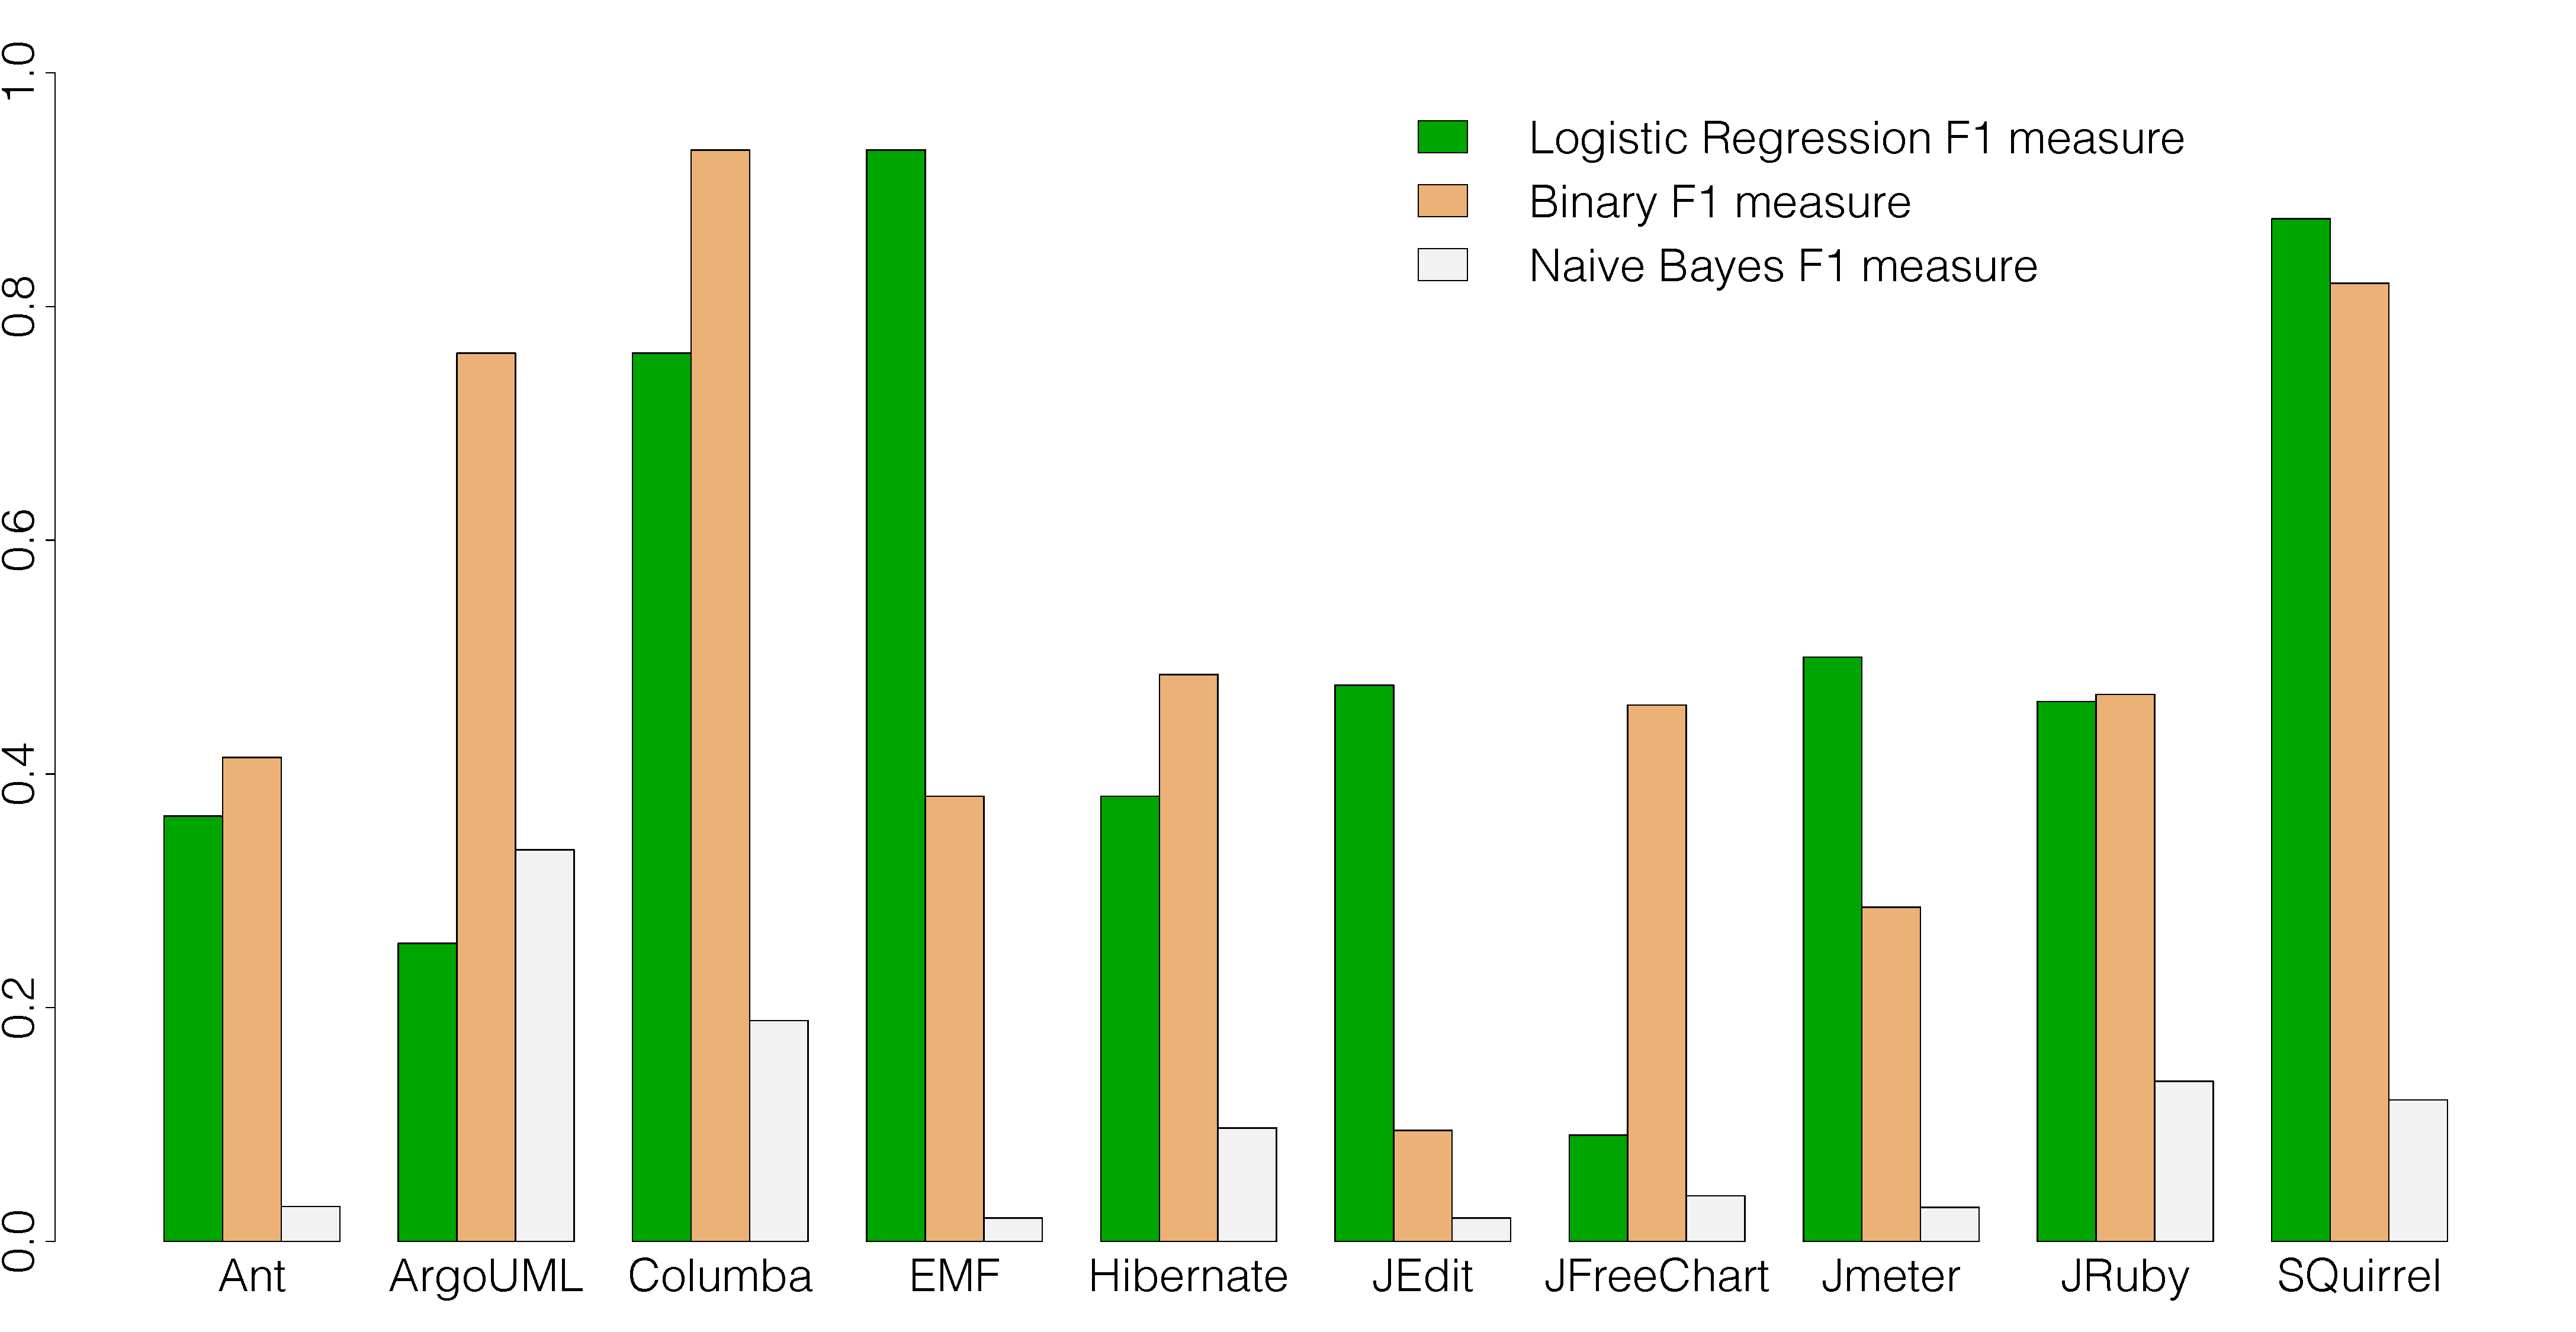
\includegraphics[width=0.48\textwidth]{figures/classifier_algorithms_comparison_requirement.pdf}
  \label{fig:algorithms_comparison_requirement}}
  \caption{Classification algorithms performance comparison}
  \label{fig:algorithms_comparison}
\end{figure*}

In this paper we propose an approach to identify \SATD comments using the Stanford Classifier. This tool, once trained correctly, can automatically classify natural language text. We create a training dataset of \SATD comments and analyzed the classification performance across ten open source projects. In RQ1, we show that our approach can outperform the current state-of-the-art in 10 out of 10 projects while identifying design and requirement debt. However, is not clear the reason why our approach was not equally effective across all projects. For example, JEdit has the worst F1 measure of all projects while classifying requirement \SATD.

\subsection{Investigating Outlier Projects}
By investigating JEdit comments, we notice two main reasons: first, the project has 10,322 comments. Of those only 14 are requirement \SATD. The data distribution represents a challenge to the classification. Even though the dataset is very unbalanced our precision was 0.125, which compared with the random classifier baseline precision of 0.001, shows that our approach is still much more useful. Second, most requirement \SATD comments in this project are in the middle of long comments. Since our approach create a high number of prediction features for \SATD comments and also for without technical debt comments, long comments have more chances to match a higher number of without technical debt features. Therefore, long comments can generate `noise' that hinders the classification performance. One possible way to reduce this effect is through the addition of more similar data, as the addition of more similar data can change the prediction features generated by the classifier. 

\emad{I do not see the point of the 2 paragraphs below}

\emad{begin: remove} Intuitively we know that each project has its own particularities, and that each group of developers, must often, create a unique way to communicate their concerns with each other. This unique trait of source code comments is inherited from the natural language itself and renders the fully automated prediction of every single \SATD very unlikely. Even when analyzing a old aged project, changes in the context of the application and turnover of developers can reflect changes in the way that source code comments are written. We can notice the impact of these particularities on the detailed performance analysis conducted in RQ3, where we can notice that the addition of more comments can eventually decrease the F1 measure performance.


For a great portion of \SATD comments there are common traits. Words as `workaround', `hack' are commonly imbued with criticism and the developers sense that this is not the appropriate solution for the problem in hand. However, relying just in these words for the identification of \SATD is not good enough as shown in Figures \ref{fig:f1_measure_comparison_design_debt} and \ref{fig:f1_measure_comparison_requirement_debt}. Therefore, NLP techniques, as proposed in our work, are needed in order to effectively identify \SATD comments.
\emad{end: remove}

\subsection{Investigating the Impact of the Underlying Classifier of the NLP Classification}

In our work, all the classification done by the Stanford Classifier used a Logistic Regression classifier. However, would be interesting to see how other  algorithms perform when classifying our dataset. Then, we choose two other algorithms to execute the classification with: Naive Bayes generative classifier and Binary classifier.

Figures \ref{fig:algorithms_comparison_design} and \ref{fig:algorithms_comparison_requirement} compare the performance between the three different algorithms. We find that the Naive Bayes has the eorst average F1-measure of 0.308 and 0.058 for design and requirement technical debt, respectively. The reason behind the low F1-measure average is that the Naive Bayes algorithm favors recall at the expense of precision \emad{we need a citation for this claim}. For example, while classifying design debt, the average recall was of 0.847 and precision 0.195. The two other algorithms present more balanced results compared to Naive Bayes, and the difference in performance between them is not as accentuate. The Logistic Regression classifier achieved F1-measures of 0.620 and 0.403, while the binary classifier F1-measures for design and requirement \SATD is 0.634 and 0.400, respectively. 

Although the Binary classification has a slightly better performance, for our research purpose, the Logistical Regression algorithm provide more insightful features as outcome. These features were analyzed and presented in RQ2. 

\subsection{Textual Similarity for Design and Requirement Debt}
%Through this study we shown which words can be used to identify design technical debt in the comments. We also find how effective this approach is. Accordingly to the findings of this study, the recall can suffer with the different domains of each project. Besides that, we would like to know how well our approach compares in finding design technical debt with other techniques that are well-known and accepted in the software engineering research community.Thus, we open two discussion sections below to address these subjects.
%
%\subsection{How the proposed dictionary behaves considering different projects domains}
%\emad{Can we add a table that has the results for all the projects.}
%As shown in the study case, is possible to observe that the recall of our approach can reach low percentages while the precision is quite hight, we argue that one possible reason is the impact that specific domain comments has on a generic dictionary to identify technical debt. As intuitively expected, comments within a specific project tend to be closely related with the domain of the application. Sometimes these comments become so specific that makes the automated detection difficult using the current techniques. 
%
%Although the dictionary could by improved adding more terms in order to achieve a higher recall rate, we considered doing this a non optimal solution as it would mean changing the dictionary for each analyzed project, which considerably increases the complexity of the approach and may impact the overall precision as well. 
%
%In this study we suggest a dictionary that contains 175 different terms that can be used to identify design technical debt from the comments with a hight precision rate (85.58\%). Based on our findings, different projects domains should not impose a precision rate drop although further work may be necessary in order to achieve a hight recall rate.
%
%\subsection{Identify Applicable Automated Refactoring Opportunities to Mitigate \SADTD}
%%\rqiii
%%
%%\noindent \textbf{Motivation:} Software engineers practitioners dedicate a large amount of time, effort and money in order to maintain their source code in a good working condition. As well the research community invest a loot \emad{loot?} of resources in this subject, as a result different tools were developed to support code maintenance and more specifically tools that helps the software engineer to analyze and improve the design of existent code. We want to analyze the overlap between self-admitted design technical debt and automated refactoring opportunities that our approach can reveal. That could show us that refactoring opportunities tools can take advantage of this light weight approach to detect design flaws in combination of the other analysis already implemented. 
%%\emad{I would say that we should say 1. We know that design technical debt exists, 2. so how can we deal with it?, 3. one way is to use automated approaches, such as refactoring tools. 4. Now we examine how well these refactoring tools can help us deal with this design debt.}
%%
%%
%%\noindent \textbf{Approach:} In the a previous section we shown how to use JDeodorant to extract the comments for our analysis, now we will see in detail how to use it to check for refactoring opportunities. \emad{Here, I would just say we use JDeodorant to help us determine these automated refactorings}
%%
%%JDeodorant can analyze the source code and suggest refactoring opportunities within these categories:Extracting Class refactoring opportunities, Type Check Elimination refactoring opportunities, Extract Method refactoring opportunities and Move Method refactoring opportunities \emad{maybe we should add a brief description of each of these in a table}. The tool also provides an interface that enables our program to call JDeodorant and check for the mentioned refactorings opportunities in the desired  fragment of code. This interface can be found in JDeodorant source code in the Standalone class. 
%%
%%We took advantage of this functionality to implement in our extraction tool one feature that analyses the comments that where identified as design technical debt. The Standalone mode of JDeodorant expects one `ClassObject` object as parameter in order to search for each one of the four available refactorings. So the first step for us is to associate the `CommentClass` of our extraction tool with the `ClassObject` expected by JDeodorant. Then we check if the refactorings opportunities suggested by the tool is in the same method that our design technical debt comment was found and store this result in the database \emad{we should discuss this in the threats section,i.e., our accuracy here is at the granularity of the method}.
%%
%%To identify if the method found in the refactoring opportunities is the same as the one that we found in our extraction tool we compare them using the method signature. We did small modifications in our version of JDeodorant to achieve that. We added methods to support this comparison for Extract Method refactoring candidates and for Extract Class refactoring candidates. The only exception is for Type Checking refactoring candidates that we check the name of the method instead of the method signature.   
%%
%%\par \noindent \textbf{Results:} In total our approach could identify 964 comments as containing design technical debt, JDeodorant found refactoring opportunities for 24.59\% of the comments, which means 237 comments. \emad{Please elaborate on this and say the type of refactoring and just elaborate on the results in general, e.g., what type of design debt can be automatically refactored, etc.}
%%
%%\emad{The idea here is to say that apron. 24.6\% of the self-admitted technical debt can be addressed by automatic refactorings.}
%%
%%\conclusionbox{Our findings shows that JDeodorant found refactoring candidates for 24.59\% of the methods classified as design technical debt by our approach.}
%
%\subsection{How our approach compares to state of the art design technical debt detection}
%\emad{Perhaps we can elaborate more on the type of stuff we find vs. what they find. We can also give real examples to help prove our point.}
%Design Technical has been studied before from several perspectives but, until now, not the developers comments perspective. Therefore, we would like to compare how our proposed approach compares with proved techniques used in previous studies \cite{Zazworka2011MTD}. Zazworka used Marinescus \cite{Marinescu2004ICSM} detection strategies to identify god classes as they are a strong indicator to design technical debt. Thus, we used the same detection strategies to identify the god classes in each one of our projects and then we  compare the overlap with design technical debt comments found on these files.
%
%As shown in Table~\ref{tab:godclasscomparison}, there is few to none overlap between the two approaches in the majority of the compared projects. We argue then that we are essentially identifying different classes with design technical debt based on the knowledge of the developers. Therefore we suggest that combining both approaches is a better solution than using just one of them.  

\section{Related Work}
\label{sec:related_work}

Our work uses code comments to detect \SADTD. Therefore, we divide the related work into three categories: source code comments, technical debt, and code smell detection.

\subsection{Source Code Comments}

A number of studies examined the co-evolution of source code comments and the rationale for changing code comments. For example, Fluri \textit{et al.}~\cite{Fluri2007WCRE} analyzed the co-evolution of source code and code comments, and found that 97\% of the comment changes are consistent. Tan \textit{et al.}~\cite{Tan2012ICST} proposed a novel approach to identify inconsistencies between Javadoc comments and method signatures. Malik \textit{et al.} \cite{Malik2008ICSM} studied the likelihood of a comment to be updated and Found that   call dependencies, control statements, the age of the function containing the comment, and the number of co-changed dependent functions are the most important factors to predict comment updates.

Other work used code comments to understand developer tasks. For example. Storey \textit{et al.}~\cite{Storey2008ICSE} analyzed how task annotations (e.g., TODO, FIXME) play a role in improving team articulation and communication. The work closest to ours is the work by Potdar and Shihab~\cite{Potdar2014ICSME}, where code comments were used to identify technical debt. 

Similar to some of the prior work. we also use source code comments to identify technical debt. However, our main focus is on the detection of \SADTD. As we have shown, our approach yield different and better results in detection \SADTD. Furthermore, we propose comment patterns, that are derived from source code comments, to detect \SADTD.

%Our goal is to find comment patterns that can recover such information and compute the accuracy of those patterns.
%in contrast to prior work that identifies comments that needs to be updated.
%Second, we use task annotations in combination with word patterns in the comments to enhance the identification of \SADTD.

\subsection{Technical Debt}

A number of studies have focused on the study of, detection and management of technical debt. Much of this work has been driven by the Managing Technical Debt Workshop effort. Fore example, Seaman \textit{et al.}~\cite{Seaman2011}, Kruchten \textit{et al.}~\cite{Kruchten2013IWMTD} and Brown \textit{et al.}~\cite{Brown2010MTD} make several reflections about the term technical debt and how it has been used to communicate the issues that developers find in the code in a way that managers can understand. Other work focused on the detection of technical debt. Zazworka \textit{et al.} \cite{Zazworka2013CSE} conducted an experiment to compare the efficiency of automated tools in comparison with human elicitation regarding the detection of technical debt. They found that there is small overlap between the two approaches, and thus it is better to combine them than replace one with the other. In addition, they concluded that automated tools are more efficient in finding defect debt, whereas developers can realize more abstract categories of technical debt.
In follow on work, Zazworka \textit{et al.}~\cite{Zazworka2011MTD} conducted a study to measure the impact of technical debt on software quality. They focused on a particular kind of design debt, namely God Classes. They found that God Classes are more likely to change, and therefore, have a higher impact in software quality. Fontana \textit{et al.}~\cite{Fontana2012MTD} investigated design technical debt appearing in the form of code smells. They used metrics to find three different code smells, namely God Classes, Data Classes and Duplicated Code. They proposed an approach to classify which one of the different code smells should be addressed first, based on a risk scale. Also related here, Potdar and Shihab~\cite{Potdar2014ICSME} used code comments to detect technical debt.They extracted the comments of four projects and analyzed more than 101,762 comments to come up with 62  patterns that indicates self-admitted technical debt. Their findings show that 2.4\% - 31\% of the files in a project contain self-admitted technical debt.

Our work is different from the work that uses code smells to detect design technical debt since we use code comments to detect design technical debt. Also, our focus is on \emph{self-admitted} design technical debt. As we have shown in the discussion section, there is very little overlap between the \SADTD that our approach detects and the design technical debt detected using code smells (in particular God classes).

% First, we propose an approach to identify \SADTD~comments specifically, instead of the more general approach that takes in consideration all kinds of TD. We also evaluate this approach in means of precision and recall, which corroborate with prior findings especially the work in \cite{Potdar2014ICSME}. Second, our study proposes a light-weight technique to find \SADTD~using source code comments.
%in addition to that we complement the proposed technical debt landscape giving a taxonomy of \SADTD~and we also discuss how much of these \SADTD~can me automatically refactored by tools.

\subsection{Code Smell Detection}

Other work build tools and techniques to facilitate the detection of code smells. Moha \textit{et al.} \cite{Moha2010TSE} proposed DECOR, a tool that incorporates a set of techniques to identify code smells in the source code. They used a domain specific language (DSL) to specify code smell detection rules. Their approach automatically generates detection algorithms based on the code smell specifications. They evaluated their techniques in 11 open-source projects and found that DECOR can effectively detect code smells, with an average precision of 60.5\% and recall of 100\%. Palomba \textit{et al.} \cite{Palomba2013} proposed an approach to identify code smells based on the evolution of the source code. In order to do that they mined the history change from the source code repository and then they searched for bad smells. They show that using their approach (HIST), they are able to identify 5 different bad smells. Tsantalis \textit{et al.} \cite{Tsantalis2009TSE} proposed a methodology that identified Feature Envy bad smells and evaluated the refactoring to remove the bad smell.

Our work complements the prior work on code smell detection, since we propose the use of code comments to detect \SADTD. In particular, we propose 176 comment patterns to identify \SADTD. Analyzing the source code comments using our approach in addition to the source code analysis techniques already employed in prior work can lead to optimal results, since our analysis showed that our approach yields results that are complementary to what code smell approaches detects.

\section{Threats to validity}
\label{sec:threats_to_validity}


\noindent\textbf{Internal validity} consider the relationship between theory and observation, in case the measured variables do not measure the actual factors. The comment patterns derived by us heavily relied on manual analysis of the code comments from Apache Ant. Like any human activity, our manual classification is subject to personal bias. To reduce this bias, any comment that was questionable was discussed between the three authors of the paper. When performing our study, we used well-commented Java projects. Since our technique heavily depends on code comments, our results and performance measures may be impacted by the quantity and quality of comments in a software project.  

When we investigate if there are refactoring recommendations to address the detected \SADTD, we essentially examine if the methods in which design debt is found participate in any of the refactoring opportunities suggested by JDeodorant.
The presence of a refactoring opportunity for a given method, may not necessarily address the same kind of design debt described in the comment. In the future, we plan to investigate in a more fine-grained level the applicability of the suggested refactorings to \SADTD.

When calculating the precision and recall values, we needed to manually examine the comments and label them as related to \SADTD or not. Any errors in our labeling may impact the precision and recall values reported.
 
%To mitigate this risk, we ask for other reviewers to examine samples of the classified data. Changing this dataset may impact our finding. 

\noindent \textbf{External validity} consider the generalization of our findings. All of our findings were derived from comments in open source projects. To minimize external validity, we chose open source projects from different domains. That said, our results may not generalize to other open source or commercial projects. In particular, our results may not generalize to projects that have a low number or no comments.
 
%In this study we analyzed open source projects from different domains, therefore our findings may not generalize to other open source or commercial projects. 
%There are different domains to be explored and projects can have a variety of factors that can impact the number of comments like size of project, domain complexity number of contributors etc and therefore our results may not generalize to all of them.

\section{Conclusion and Future work}
\label{sec:conclusion}

The term Technical Debt is often used to express some kind of inadequacy in the source code in a way that is understandable to management. But this metaphor can represent many different kind of things, inappropriate or temporary solution to meet a deadline, error prone code, lack of tests and documentation and even design flaws or workarounds. Sometime, developers are aware of these problems and they may express their concern through comments in the source code. Therefore, in this study we propose an approach to identify such comments in the source code. Our findings show that:

\begin{itemize}
\item The derived 176 comment patterns can be used to effectively identify \SADTD, with precision values ranging between 74.07-96.30\% and recall values ranging between 10.87-83.87\%.
\item The design technical debt identified by out approach is different than the design technical debt detected through code smells. 

\item Approximately 24.58\% of the detected \SADTD can be automatically refactored with automated refactoring tools.

\end{itemize} 

%During this study we also presented 3 Heuristics and one post-processing technique to eliminate irrelevant comments, the development of a taxonomy and a 176 \SADTD~patterns to address design technical debt and finally we shown the effectiveness of refactoring tools dealing with design technical debt. 

We believe that our study lays the ground work for future work in the area of self-admitted technical debt. In the future, we plan to explore Natural Language Processing techniques in order to improve the detection of \SADTD across projects. Furthermore we plan to expand the current taxonomy to include more categories of technical debt like defect and test technical debt. Finally, we plan to explore the use of our technique to possibly rank refactoring candidates suggestions from automated tools based on the type of technical debt. 

\bibliographystyle{IEEEtran}
\balance
\bibliography{design_td}



\appendix{}
\label{sec:appendix}

Table~\ref{tab:comment_patterns} lists all of the comment patterns derived in our study. If the paper is accepted, this appendix will be provided through an online link. We include this appendix, which will be removed later, so that reviewers need not go to an online link during the review process. Online links have been discouraged in the past during the review process since they may indicate the identity of the anonymous reviewers.


\begin{table*}[thb!]
	\begin{center}
		\caption{The Derived 176 Comment Patterns that Indicate \SADTD}
		\label{tab:comment_patterns}
		\begin{tabular}{l| l| l| l }
			\toprule
			`\%future\%may\%'            & `\%perhaps\%elsewhere\%'    & `\%hard\%coding\%'            & `\%todo\%complex\%'       \\
			`\%future\%better\%'         & `\%rather\%complex\%'       & `\%kludge\%'                  & `\%fixme\%complex\%'      \\
			`\%future\%enhance\%'        & `\%held\%?\%'               & `\%todo\%public\%'            & `\%xxx\%complex\%'        \\
			`\%future\%change\%'         & `\%though\%unused\%'        & `\%fixme\%public\%'           & `\%consistency\%sake\%'   \\
			`\%quick\%fix\%'             & `\%todo\%don\%know\%'       & `\%xxx\%public\%'             & `\% lack \%broke\%'       \\
			`\%temporary\%until\%'       & `\%fixme\%don\%know\%'      & `\%messy\%'                   & `\% lack \%problem\%'     \\
			`\%place\%somewhere\%else\%' & `\%xxx\%don\%know\%'        & `\%should\%instead\%'         & `\% lack \%should\%'      \\
			`\%move\%somewhere\%else\%'  & `\%don\%know\%try\%'        & `\%this\%weird\%'             & `\%todo\% lack \%'        \\
			`\%used\%other\%place\%'     & `\%don\%know\%fail\%'       & `\%weird\%this\%'             & `\%fixme\% lack \%'       \\
			`\%it \%may \%change \%'     & `\%don\%know\%what\%'       & `\%todo\%weird\%'             & `\%xxx\% lack \%'         \\
			`\%this may change\%'        & `\%don\%know\%fix\%'        & `\%fixme\%weird\%'            & `\%todo\% long \%'        \\
			`\%todo\%can\%change\%'      & `\%not\%fond\%'             & `\%xxx\%weird\%'              & `\%fixme\% long \%'       \\
			`\%fixme\%can\%change\%'     & `\%more\%elegant\%'         & `\%todo\%availability\%'      & `\%xxx\% long \%'         \\
			`\%xxx\%can\%change\%'       & `\%clean\%way\%'            & `\%fixme\%availability\%'     & `\%todo\% large \%'       \\
			`\%not \%sure \%'            & `\%todo\%remove\%'          & `\%xxx\%availability\%'       & `\%fixme\% large \%'      \\
			`\%dependency\%cycle\%'      & `\%xxx\%remove\%'           & `\%todo\%extensibility\%'     & `\%xxx\% large \%'        \\
			`\%todo\%dependenc\%'        & `\%fixme\%remove\%'         & `\%fixme\%extensibility\%'    & `\%future\%maintenance\%' \\
			`\%fixme\%dependenc\%'       & `\%todo\%don\%want\%'       & `\%xxx\%extensibility\%'      & `\%todo\%maintenance\%'   \\
			`\%xxx\%dependenc\%'         & `\%fixme\%don\%want\%'      & `\%sacrifice\%flexibility\%'  & `\%fixme\%maintenance\%'  \\
			`\%code\%cop\%from\%'        & `\%xxx\%don\%want\%'        & `\%todo\%flexibility\%'       & `\%xxx\%maintenance\%'    \\
			`\%copied\%code\%'           & `\% fix \% for \%'          & `\%fixme\%flexibility\%'      & `\%todo\%unused\%'        \\
			`\% any \%reason\%'          & `\% fix for \%'             & `\%xxx\%flexibility\%'        & `\%fixme\%unused\%'       \\
			`\%wrong\%place\%'           & `\%irritating\%'            & `\%todo\%scalability\%'       & `\%xxx\%unused\%'         \\
			`\%hairy\%'                  & `\%todo\%duplicat\%'        & `\%fixme\%scalability\%'      & `\%currently\%unused\%'   \\
			`\%instead\%could\%'         & `\%fixme\%duplicat'         & `\%xxx\%scalability\%'        & `\%unused\%delete\%'      \\
			`\%ugly\%'                   & `\%xxx\%duplicat\%'         & `\%security\%compatibility\%' & `\%unused\%currently\%'   \\
			`\%todo\%avoid\%'            & `\%why\%not\%'              & `\%security\%never\%'         & `\%such\%bad\%'           \\
			`\%fixme\%avoid\%'           & `\%rethink\%'               & `\%todo\%security\%'          & `\%todo\%bad\%'           \\
			`\%xxx\%avoid\%'             & `\%rework\%'                & `\%fixme\%security\%'         & `\%fixme\%bad\%'          \\
			`\%should\%avoid\%'          & `\%pointless\%'             & `\%xxx\%security\%'           & `\%xxx\%bad\%'            \\
			`\%pathological\%'           & `\% not \%nice\%'           & `\%todo\%ambiguous\%'         & `\%todo\%clone\%code\%'   \\
			`\%stolen\%'                 & `\%hack\%'                  & `\%fixme\%ambiguous\%'        & `\%fixme\%clone\%code\%'  \\
			`\%not\%well\%formed\%'      & `\%only\%developer\%know\%' & `\%xxx\%ambiguous\%'          & `\%xxx\%clone\%code\%'    \\
			`\% no \%sense\%since\%'     & `\% use \% help\%'          & `\%todo\% big \%'             & `\% dead \%code\%'        \\
			`\%without\%notic\%'         & `\%hammer\%'                & `\%fixme\% big \%'            & `\%crappy\%design\%'      \\
			`\%brittle\%'                & `\%todo\%redundant\%'       & `\%xxx\% big \%'              & `\%design\%flaw\%'        \\
			`\%really\%necessary\%'      & `\%fixme\%redundant\%'      & `\% big \% mess \%'           & `\% todo\% design \%'     \\
			`\%cares\%'                  & `\%xxx\%redundant\%'        & `\%clean\%needed\%'           & `\%fixme\%design\%'       \\
			`\%no idea\%'                & `\%for\%some\%reason\%'     & `\%should\%clean\%'           & `\% xxx \%design\%'       \\
			`\%idea?\%'                  & `\%alternatively\%could\%'  & `\%todo\%clean\%'             & `\%redesign\%'            \\
			`\%doing?\%'                 & `\%technically\%'           & `\%fixme\%clean\%'            & `\%todo\%magic\%'         \\
			`\%todo\%elsewhere\%'        & `\% forces \%us\%'          & `\%xxx\%clean\%'              & `\%fixme\%magic\%'        \\
			`\%fixme\%elsewhere\%'       & `\%better\%way\%'           & `\%due\%complex\%'            & `\%xxx\%magic\%'          \\
			`\%xxx\%elsewhere\%'         & `\%hard\%coded\%'           & `\%way\%complex\%'            & `\%smell\%'               \\ 
			\bottomrule
		\end{tabular}
	\end{center}
\end{table*}

\end{document}
